% !TeX spellcheck = sl_SI
\documentclass[12pt,a4paper,twoside]{article}
\usepackage[utf8]{inputenc}

\newcommand{\program}{Računalništvo in matematika}
\newcommand{\imeavtorja}{Anže Marinko}
\newcommand{\imementorja}{izr.~prof.~dr.~Iztok Lebar Bajec}
\newcommand{\imesomentorja}{doc.~dr.~Jure Demšar}
\newcommand{\naslovdela}{Vodenje psa ovčarja z uporabo umetne inteligence}
\newcommand{\letnica}{2021}
\newcommand{\opis}{Delo obravnava simuliranje gibanja ovc in čim učinkovitejše vodenje psa ovčarja s pomočjo umetne inteligence.}
\newcommand{\kljucnebesede}{umetna inteligenca\sep problem vodenja ovčarja\sep sodelovanje\sep genetski algoritmi\sep spodbujevano učenje\sep agenti}
\newcommand{\keywords}{artificial intelligence\sep shepherding problem\sep cooperation\sep genetic algorithms\sep reinforcement learning\sep agents}
\newcommand{\organization}{Univerza v Ljubljani, Fakulteta za matematiko in fiziko, Fakulteta za računalništvo in informatiko}
\newcommand{\sep}{, }
\newcommand{\literatura}{../literatura}

\usepackage{bibentry}
\nobibliography{\literatura}
\newcommand{\plancite}[1]{\item[\cite{#1}] \bibentry{#1}}
\usepackage{filecontents}
\usepackage{silence} \WarningFilter{latex}{Overwriting file}
\begin{filecontents*}{\jobname.xmpdata}
	\Title{\naslovdela} \Author{\imeavtorja} \Keywords{\kljucnebesede} \Subject{matematika} \Org{\organization}
\end{filecontents*}

\usepackage[a-1b]{pdfx}
\hypersetup{bookmarksopen, bookmarksdepth=3, colorlinks=true, linkcolor=black, anchorcolor=black, citecolor=black, filecolor=black, menucolor=black, runcolor=black, urlcolor=black, pdfencoding=auto, breaklinks=true, psdextra}

\usepackage[slovene]{babel}
\usepackage[T1]{fontenc}
\usepackage{amsmath,amssymb,amsfonts,amsthm}
\usepackage{graphicx}
\usepackage{emptypage}
\usepackage{units}
\usepackage{makeidx}
\makeindex
\usepackage[top=3cm, bottom=3cm, inner=3.5cm, outer=2.5cm, footskip=40pt]{geometry}

% Za pisanje psevdokode
\usepackage{algpseudocode}  % za psevdokodo
\usepackage{algorithm}
\floatname{algorithm}{Algoritem}

\addto\captionsslovene{\renewcommand{\listtablename}{Kazalo tabel}}
\setlength{\overfullrule}{50pt}
\pagestyle{plain}
\theoremstyle{definition}
\newtheorem{definicija}{Definicija}[section]
\newtheorem{primer}[definicija]{Primer}
\newtheorem{opomba}[definicija]{Opomba}
\newtheorem{aksiom}{Aksiom}

\theoremstyle{plain}
\newtheorem{lema}[definicija]{Lema}
\newtheorem{izrek}[definicija]{Izrek}
\newtheorem{trditev}[definicija]{Trditev}
\newtheorem{posledica}[definicija]{Posledica}

\numberwithin{equation}{section}
\newcommand{\R}{\mathbb R}
\newcommand{\N}{\mathbb N}
\newcommand{\Z}{\mathbb Z}
\renewcommand{\C}{\mathbb C}
\newcommand{\Q}{\mathbb Q}
\makeatletter \g@addto@macro\bfseries{\boldmath} \makeatother
\addto\captionsslovene{\renewcommand{\listfigurename}{Kazalo slik}}

\begin{document}

\pagenumbering{roman}
\thispagestyle{empty}
\noindent{\large UNIVERZA V LJUBLJANI\\[1mm] FAKULTETA ZA MATEMATIKO IN FIZIKO\\[1mm] FAKULTETA ZA RAČUNALNIŠTVO IN INFORMATIKO\\[5mm] \program\ -- 2.~stopnja}
\vfill

\begin{center}
  \large \imeavtorja\\[3mm] \Large \textbf{\MakeUppercase{\naslovdela}}\\[10mm] \large Magistrsko delo \\[1cm] Mentor: \imementorja \\[2mm] Somentor: \imesomentorja
\end{center}
\vfill
\noindent{\large Ljubljana, \letnica}
\cleardoublepage


\pdfbookmark[1]{Zahvala}{zahvala} %
\section*{Zahvala}
\setlength{\parskip}{0.8em}

Hvala mentorju izr.~prof.~dr.~Iztoku Lebarju Bajcu in somentorju doc.~dr.~Juretu Demšarju za usmerjanje in pomoč pri raziskovanju in pisanju. Zahvaljujem se tudi vsem ostalim profesorjem, ki so me v teh letih pripravljali in me navduševali nad matematičnimi in računalniškimi tematikami, ki mi bodo koristile v življenju.

Zahvaljujem se svojim staršem, Tonetu in Mateji, bratom Luku, Janezu, Denisu, Matevžu in Alenu ter sestrama Sari in Ani, za zgled in podporo pri učenju ter študijskemu delu vsa ta leta. Hvala tudi moji zaročenki Karolini za spodbudne besede in da mi v vsem stoji ob strani. Hvala vsem prijateljem, soskavtom in sopevcem za navdihujoče okolje.

Hvala Ani Kepic za slovnični pregled dela.
\setlength{\parskip}{0.1em}

\cleardoublepage
\pdfbookmark[1]{\contentsname}{kazalo-vsebine}
\tableofcontents
\cleardoublepage
\pdfbookmark[1]{\listfigurename}{kazalo-slik}
\listoffigures
\pdfbookmark[1]{\listtablename}{kazalo-slik}
\listoftables
\cleardoublepage

\section*{Program dela}
\addcontentsline{toc}{section}{Program dela}

V magistrski nalogi bo kandidat preučeval smiselnost uporabe metod umetne inteligence za učenje vodenja psa ovčarja. V danem problemu je cilj psa ovčarja, da skupino ovc čim hitreje privede v hlev.

V prvi fazi naloge bo kandidat pridobil oziroma osvežil potrebna znanja. Simulacije bo sprogramiral v orodju Unity. Okolje se primarno uporablja za razvoj računalniških iger, a je več kot primerno tudi za izdelavo raznih vizualnih simulacij~\cite{Demsar}. V sklopu učenja orodja Unity, se bo kandidat moral naučiti tudi programskega jezika C\#.

Za učenje vodenja psa bomo uporabili dva različna pristopa. Prvi pristop so genetski algoritmi, pri njih se entitete učijo oziroma napredujejo skozi poenostavljeno simuliranje naravne evolucije~\cite{natureOfCode}. Za drugi pristop smo izbrali bolj moderen in kompleksen programski paket imenovan ML Agents.  Metoda je osnovana na spodbujevanem učenju in je integrirana v orodje Unity.

Naučeno vodenje psa bomo temeljito evalvirali. Uspešnost naučenega vodenja v obeh primerih (genetski algoritmi in ML Agents) bomo primerjali z ročno sprogramiranim vodenjem~\cite{Stroembom}. Primerjavi bomo izvedli na dveh različnih modelih vedenja ovc, na enostavnem modelu~\cite{Stroembom} ter na modelu zgrajenem s pomočjo dejanskega gibanja ovc v naravi~\cite{Ginelli}.

\section*{Osnovna literatura}
% po pomembnosti:
\begin{itemize}
  \plancite{Stroembom}
  \plancite{Ginelli}
  \plancite{natureOfCode}
  \plancite{Demsar}
\end{itemize}

\vspace{.5cm}
\hspace*{\fill} Podpis mentorja: \phantom{prostor za podpis}

\vspace{1.5cm}
\hspace*{\fill} Podpis somentorja: \phantom{prostor za podpis}

\cleardoublepage

\let\oldsection\section
\def\section{\cleardoublepage\oldsection}
\pdfbookmark[1]{Povzetek}{abstract}

\begin{center}
\textbf{\naslovdela} \\[3mm]
\textsc{Povzetek} \\[2mm]
\end{center}

V naravi lahko en sam ovčar zbere in vodi čredo več sto ovc, ljudje pa si želimo zbirati, voditi ali preusmerjati tudi druge vrste živali. V bližini letališč imajo letala pogosto težave z jatami ptic, ki letalom med drugim povzročajo škodo na motorjih ali celo strmoglavljanja. V ta namen so že mnogi raziskovali različne modele vodenja s pomočjo umetne inteligence, da bi se podobnih problemov lahko lotili z roboti ali droni. Uporaba pametnih ovčarjev bi lahko prav prišla tudi pri zbiranju razlite nafte na vodi ali pri vodenju panične množice ljudi na varno v kriznih situacijah.

V tem delu študiramo različne modele gibanja ovc, razvijamo model vodenja in ga še izboljšamo z metodami umetne inteligence. Pri tem predlagamo rešitve za različne težave, ki se pri učenju pojavljajo. Razviti želimo namreč model, po katerem ovčarji kar se da hitro v stajo prepeljali celotno čredo. Osnovnemu modelu vodenja najprej dodamo sodelovanje več ovčarjev, nato najdemo dobre parametre modela za izbrane velikosti črede in število ovčarjev. Na koncu razvijemo model, pri katerem se na podlagi izbranih informacij ovčar sproti odloča o vrednostih parametrov.

\vfill
\begin{center}
\textbf{Guide a sheepdog using artificial intelligence} \\[3mm]
\textsc{Abstract}\\[2mm]
\end{center}

In the wild, a single shepherd can gather and lead a herd of hundreds of sheep, and people want to collect, lead or divert other species of animals as well. In the vicinity of airports, aircraft often have problems with flocks of birds, causing them damage to their engines or even crashes. Many have already researched various models of guidance using artificial intelligence in order to be able to tackle similar problems with robots or drones. The use of smart shepherds could also come in handy when collecting spilled oil on the water or when leading a panicked crowd of people to safety in crisis situations.

In this part, we study different models of sheep movement, develop a management model and further improve it with artificial intelligence methods. We propose solutions to various problems that arise in learning. Namely, we want to develop a model according to which shepherds transport the entire herd to the stable as quickly as possible. We first add the participation of several shepherds to the basic management model, then we find good model parameters for the selected herd sizes and number of shepherds. Finally, we develop a model in which the shepherd decides on the values of parameters on the basis of selected information.

\vfill\noindent
\textbf{Math.~Subj.~Class.~(2020):} 68T20, 68T42, 70E55, 70E60 \\[1mm]
\textbf{Ključne besede:} \kljucnebesede \\[1mm]
\textbf{Keywords:} \keywords

\cleardoublepage
\setcounter{page}{1}
\pagenumbering{arabic}
\setlength{\parskip}{0.8em}

% ============= Vsebinski del ===========================

\section{Uvod}

Živali se pogosto zbirajo in gibljejo v bolj ali manj strnjenih skupinah. Skupini sesalcev iste vrste, posebej iz reda kopitarjev, rečemo čreda, skupina ptic ali rib je jata. Sicer pa se živali zbirajo tudi v tako imenovane trope, roje ipd. Z zbiranjem v skupino je posamezna žival bolj varna pred plenilci in se tudi lažje pari za ceno večje opaznosti skupine v primerjavi s posamezno živaljo, hitrejšim prenosom bolezni znotraj skupine ter za ceno manjše količine hrane na posamezno žival v njeni okolici.

Človek je za varovanje, zbiranje in vodenje črede ovc, da se je ta varno in hitreje premikala po pašniku ter tako varno popasla večje območje, udomačil pse ovčarje. Ovčarjevo obnašanje je pravzaprav prevzgojeno plenilsko obnašanje. V Sloveniji je edina avtohtona pasma kraški ovčar ali kraševec, ki ga je omenil že Janez Vajkard Valvasor v knjigi Slava Vojvodine Kranjske. Je pa kraški ovčar po značaju bolj pastirski pes, kar pomeni, da je umirjen, a ves čas pozoren na nevarnosti, saj bolj kot zbira čredo varuje~\cite{krasevec}.
Ovčarji so sami sposobni zbrati in voditi veliko čredo, lahko celo več sto ovc, saj jim pri tem ključno pomaga močan čredni nagon pri ovcah in strah ovc pred njimi. Podobno situacijo, kjer se skupina živali, ljudi ali drugih delcev (z eno besedo agentov) giblje v podobni smeri, opazimo tudi drugje v naravi in včasih bi nam koristilo, da bi imeli udomačeno žival tudi za druge podobne probleme. 

Tak primer so recimo jate ptic v okolici letališč. Jata ptic namreč lahko ob trku poškoduje letalo, kar se večinoma zgodi ob vzletanju ali pristajanju, saj večina ptic leti nizko, kar lahko vodi celo do strmoglavljenja. V ZDA naj bi bilo med letoma 1990 in 2010 že samo prijavljenih trkov s pticami kar 121 000, na svetu pa naj bi bilo med letoma 1988 in 2012 najmanj 200 smrti zaradi tovrstnih nesreč~\cite{letalske-nesrece}. Leta 2019 je v Etiopiji zaradi ptic v eni sami letalski nesreči umrlo 157 ljudi~\cite{letalske-nesrece2}. Najbolj znana nesreča s srečnim izidom pa je bila "Čudež na Hudsonu" v New Yorku leta 2009, ko je v nesreči dobro minuto po vzletu prišlo do trka z jato ptic. Preživelo je vseh 155 potnikov~\cite{letalske-hudson}. Pilot je kljub odpovedi obeh motorjev pristal in to kar na reki Hudson. O tem dogodku je posnet tudi film Sully~\cite{letalske-sully} imenovan po tem pilotu.

Za tovrstne probleme pa žal nimamo udomačene nobene vrste živali. Ideja je, da bi jih lahko nadomestili z uporabo robotov ali dronov. Zgledovali pa bi se po psih ovčarjih. V Novi Zelandiji so leta 2020 Boston Dinamics poskusili voditi ovce s pomočjo robotskega psa~\cite{robot-sheperd} in ugotovili, da se ovce podobno kot na psa odzivajo tudi na njihovega robota. Ta robot deluje brez človeškega sodelovanja, ampak ga za vodenje črede niso posebno izurili, mi pa si želimo najti uspešen algoritem, ki bo sposoben učinkovito pripeljati vse ovce v stajo v čim krajšem času. Uporaba pametnih ovčarjev robotov razvitih na podoben način bi lahko prav prišla tudi pri preusmerjanju jate ptic v okolici letališč, zbiranju razlite nafte na vodi ali pri vodenju panične množice ljudi na varno v kriznih situacijah.

Na letališčih že uporabljajo različne načine za preusmerjanje ptic. Da bi ptice vodili brez sodelovanja človeka, je korejska raziskovalna skupina že razvila algoritem za preusmerjanje jate ven iz območja letališča~\cite{bird-herd, letalske-chung, letalske-chung2}. Mi pa se bomo v tem delu osredotočili na vodenje črede ovc v stajo z uporabo umetne inteligence. Z uporabo umetne inteligence bi se ovčar robot lahko učil tudi tekom dela z vrsto živali, ki se obnaša kako drugače.

\subsection{Organizacija dela}

Različni avtorji so se že lotili modeliranja gibanja ovc in psa ovčarja kot agentov. V tem delu si bomo najprej ogledali dva modela gibanja ovc, ki sta ju predstavila avtorja Str{\"o}mbom~\cite{Stroembom} in Ginelli~\cite{Ginelli} s sodelavci. Prvi model bomo tudi nekoliko spremenili, da dobimo bolj naravno gibanje in tako skupno tri modele gibanja ovc. Obnašanje agentov je po vseh treh modelih dovolj različno, da bomo s tem lahko preizkusili robustnost algoritmov vodenja psa ovčarja.

Ogledali si bomo model gibanja psa ovčarja, ki so ga predlagali avtorji članka~\cite{Stroembom}. Modelu smo dodali tudi nekaj izboljšav in sodelovanje več psov z deljenjem črede glede na Voronoieve celice. Da bi uspeh algoritma še izboljšali v smislu hitrosti in uspešnosti vodenja ovc v stajo, smo parametre modela nastavili s pomočjo genetskega algoritma, ki temelji na ideji evolucije. Parametre smo nastavili v odvisnosti od velikosti črede, modela gibanja ovc in števila psov ovčarjev.

Ker pa se število ovc na pašniku sčasoma spreminja, ko ovce pridejo v stajo, želimo parametre prilagajati glede na trenutno in ne le glede na začetno stanje. Z uporabo spodbujevanega učenja (umetna inteligenca), natančneje PPO algoritma z nevronsko mrežo, si želimo dobljeni algoritem še izboljšati. Učenje smo pospešili z demonstracijami.

Na koncu pa si bomo ogledali še program \textit{iOvčar IZIDOR} za izvajanje simulacij in učenja, ki smo ga naredili v programu Unity in za umetno inteligenco uporablja paket ML Agents. Program je napisan v programskem jeziku~\textit{C\#}. Predstavitvi programa sledi še pregled rezultatov in primerjava modelov vodenja.

\section{Obnašanje ovc}

V tem poglavju si bomo ogledali dva modela obnašanja ovc avtorjev Str{\"o}mboma s sodelavci~\cite{Stroembom} in Ginellija s sodelavci~\cite{Ginelli}. Prvi model bomo nekoliko predelali in s tem naredili še tretji model. Za učenje in testiranje ovčarjev bomo uporabili ovce po vseh treh modelih in tako preverili robustnost metode vodenja za različne vrste agentov. Ovce so na začetku naključno enakomerno neodvisno porazdeljene v krog s polmerom 50~m na sredini kvadratnega pašnika s stranico dolgo 300~m. Na sredini ene stranice je 100~m širok vhod na cilj, ki mu bomo rekli staja. Psi ovčarji bodo v simulacijah postavljeni naključno enakomerno neodvisno kamor koli na pašnik vsaj 5~m od ograje. Na sliki~\ref{fig:zemljevid} si lahko ogledamo opisano postavitev na začetku simulacije. Ovce so porazdeljene enakomerno na modrem območju in ovčarji enakomerno na svetlo zelenem območju vsaj 5~m od ograje z namenom, da na ovčarjevo gibanje ograja ne vpliva že takoj na začetku simulacije.

\begin{figure}[ht]  % ali t za na vrhu ali h! za točno tukaj
	\centering
	\includegraphics[width=0.7\textwidth]{../poglavja/images/simulacijsko_okolje.pdf}\caption[Območja simulacijskega okolja]{Prikaz območij simulacijskega okolja s pašnikom, stajo in območji porazdelitve agentov.} % narejena je s programom Inkscape
	\label{fig:zemljevid}
\end{figure}

\subsection{Strömbomov model}\label{stroembom}

Prvi in najenostavnejši model gibanja ovc, ki si ga bomo ogledali, temelji na modelu, pri katerem ima vsak agent tri območja, ki ustrezajo trem osnovnim težnjam agenta kot predlagano v~\cite{boids} (slika~\ref{fig:boids}). Osnovne težnje agenta so:
\begin{enumerate}
	\item Agent se od ostalih agentov, ki so mu preblizu, odmika za preprečevanje trkov. Območje odbijanja je izmed vseh najmanjše.
	\item Agent poravna svojo smer gibanja z drugimi agenti, ki so mu dovolj blizu. Območje poravnave je večje od območja odbijanja.
	\item Agent se približuje agentom, ki so v njegovem zaznavnem ali vidnem polju. Območje združevanja je največje.
\end{enumerate}
Od vrste živali je odvisna velikost posameznega območja in moč posamezne težnje. Model je zasnovan za ptice, a ga lahko uporabljamo tudi v ravnini. Str{\"o}mbom je s sodelavci modelu dodal še območje strahu za beg pred grožnjo oziroma ovčarjem in zanemaril območje poravnave. Območje strahu je celo večje od vidnega polja, saj ovca že na daleč psa zazna tudi zaradi njegovega oglašanja, čeprav ta še ni v njenem vidnem polju.

\begin{figure}[ht]  % ali t za na vrhu ali h! za točno tukaj
	\centering
	\includegraphics[width=0.7\textwidth]{../poglavja/images/boids.pdf}
	\caption[Območja zaznave]{Prikaz območij modela po~\cite{boids}.} % narejena je s programom Inkscape
	\label{fig:boids}
\end{figure}

\subsubsection{Odbojna sila}

Odbojna sila služi preprečevanju trkov med agenti. Za vsako ovco, ki ima v območju odbijanja vsaj eno ovco, izračunamo odbojno silo $R_i^a$, ki je enaka vsoti normaliziranih vektorjev stran od vsake izmed ovc v območju odbijanja z radijem $r_a$.
\begin{align}
\mathbf{R}_i^a = \sum_{j\not=i,~\Vert \mathbf{A}_i - \mathbf{A}_j\Vert < r_a}\frac{ \mathbf{A}_i - \mathbf{A}_j}{\Vert \mathbf{A}_i - \mathbf{A}_j\Vert}, \label{eq:stroembom-odboj}
\end{align}
kjer je $\mathbf{A}_j$ lokacija $j$-te ovce. Primer si lahko ogledamo na sliki~\ref{fig:stroembom-odboj}.

\begin{figure}[ht]  % ali t za na vrhu ali h! za točno tukaj
	\centering
	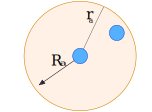
\includegraphics[width=0.49\textwidth]{../poglavja/images/stroembom_odboj.pdf}
	\caption[Odbojna sila]{Odbojna sila od ovce v območju odbijanja.} % narejena je s programom Inkscape
	\label{fig:stroembom-odboj}
\end{figure}

\subsubsection{Sila združevanja}

Ovca želi biti vedno blizu črede, saj se tako počuti varneje. Sila združevanja je kar enaka normaliziranemu vektorju usmerjenemu proti središču dela črede, ki je v njenem vidnem polju oziroma v območju združevanja s polmerom $r_d$, kot je predlagal avtor diplomskega dela~\cite{diplomska}, da bi se izognil situaciji, ko bi se ovce želele približevati ovcam, ki niso v njihovem vidnem polju, saj so avtorji lokalni center izračunavali na podlagi najbližjih $k$ sosedov za nek izbran $k$. V našem primeru pa se lahko zgodi, da ovca vidi vse ali celo nobene druge ovce. Lokalni center mase (LCM) ali lokalno težišče tako izračunamo kot
\begin{align}
\mathbf{LCM}_i = \frac{1}{k}\sum_{\Vert \mathbf{A}_i - \mathbf{A}_j\Vert < r_d} \mathbf{A}_j, \label{eq:stroembom-lcm}
\end{align}
kjer je $k$ število ovc v območju združevanja ovce $i$ vključno z njo samo in se $k$ skozi čas spreminja. Tedaj je smer sile združevanja enaka
\begin{align}
\mathbf{C}_i = \mathbf{LCM}_i - \mathbf{A}_i. \label{eq:stroembom-zdruzi}
\end{align}

Shematski prikaz sile združevanja si lahko ogledamo na sliki~\ref{fig:stroembom-zdruzi}.

\begin{figure}[ht]  % ali t za na vrhu ali h! za točno tukaj
	\centering
	\includegraphics[width=0.49\textwidth]{../poglavja/images/stroembom_zblizevanje.pdf}
	\caption[Sila združevanja]{Sila združevanja v smeri proti lokalnemu centru mase ovc v območju združevanja.} % narejena je s programom Inkscape
	\label{fig:stroembom-zdruzi}
\end{figure}

\subsubsection{Sila bega pred ovčarjem}

Ko ovca zazna grožnjo se želi od nje umakniti. Ovca beži od vseh ovčarjev, ki so v njenem območju bega s polmerom $r_s$. Smer bega izračunamo kot vsoto normaliziranih smeri stran od ovčarjev pomnoženih s faktorjem strahu pred posameznim ovčarjem
\begin{align}
\mathbf{R}_s = \sum_{\Vert \mathbf{A}_i - \mathbf{S}_j\Vert < r_s}\frac{ \mathbf{A}_i - \mathbf{S}_j}{\Vert \mathbf{A}_i - \mathbf{S}_j\Vert}\Big(\frac{ \Vert \mathbf{A}_i - \mathbf{S}_j\Vert - r_s}{r_s}\Big)^2, \label{eq:stroembom-beg}
\end{align}
kjer je $\mathbf{S}_j$ lokacija $j$-tega psa ovčarja. Faktor strahu pred posameznim ovčarjem služi temu, da se ovca bolj boji ovčarja, ki ji je bližje. Za prikaz si oglejmo sliko~\ref{fig:stroembom-beg}.

\begin{figure}[ht]  % ali t za na vrhu ali h! za točno tukaj
	\centering
	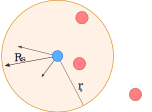
\includegraphics[width=0.49\textwidth]{../poglavja/images/stroembom_beg.pdf}
	\caption[Sila bega pred ovčarjem]{Sila bega pred dvema ovčarjema v območju strahu. Tretji ovčar je ne ogroža.} % narejena je s programom Inkscape
	\label{fig:stroembom-beg}
\end{figure}

\subsubsection{Izračun premika}

Smer gibanja $\mathbf{H}_i^\prime$ izračunamo kot uteženo vsoto vseh izračunanih normaliziranih vektorjev izračunanih po formulah~\eqref{eq:stroembom-odboj}, \eqref{eq:stroembom-zdruzi}, \eqref{eq:stroembom-beg}, normalizirane smeri v prejšnjem koraku $\hat{\mathbf{H}_{i}}$ in naključnega enotskega vektorja $\epsilon$ po formuli
\begin{align}
\mathbf{H}_i^\prime = h\hat{\mathbf{H}_{i}} + c\hat{\mathbf{C}_i} + \rho_a\hat{\mathbf{R}_i^a} + \rho_s\hat{\mathbf{R}_i^s} + e\mathbf{\epsilon}_i, \label{eq:stroembom-smer}
\end{align}
pri čemer izbrane uteži zadoščajo pogoju $\rho_a > c > \rho_s > h > e$, da ovce ostanejo na razdalji in hkrati skupaj kljub grožnji in šumu. Ničelnih vektorjev ne normaliziramo, da se med drugim izognemo begu, ko noben ovčar ni v območju strahu. Stara smer je uporabljena z namenom bolj naravnega gladkega gibanja brez ostrih zavojev. Šum z velikostjo $e$ je prisoten le z verjetnostjo $p$. Agent se ves čas giblje s konstantno hitrostjo $v$. Tako se ovca premakne na točko $\mathbf{A}_i^\prime =\mathbf{A}_i + \Delta t v\hat{\mathbf{H}_i^\prime}$, kjer je $\Delta t$ sprememba časa od prejšnjega koraka in $\hat{\mathbf{H}_i^\prime}$ normalizirana smer izračunana v~\eqref{eq:stroembom-smer}, prilagojena za izogibanje ograji na način, opisan v naslednjem razdelku.

Vrednosti parametrov, ki smo jih uporabili, si lahko ogledamo v tabeli~\ref{table:stroembom}. Večino vrednosti smo povzeli po Str{\"o}mbomu in sodelavcih~\cite{Stroembom} ter Demšarju in sodelavcih~\cite{Demsar}. Zadnja dva parametra nastopata v popravljenem modelu, opisanem v nadaljevanju.

\begin{table}[ht]
	\begin{center}
		\begin{tabular}{ c|l|c }
		\hline
		\textbf{Oznaka} & \textbf{Opis parametra} & \textbf{Uporabljena vrednost} \\ \hline  
		$r_a$ & Polmer območja odbijanja & 2~m \\ 
		$r_s$ & Polmer območja združevanja & 30~m \\ 
		$r_d$ & Polmer območja strahu & 15~m \\ 
		$\rho_a$ & Relativna moč odbojne sile & 2 \\ 
		$c$ & Relativna moč sile združevanja & 1,05 \\ 
		$\rho_s$ & Relativna moč sile bega pred ovčarjem & 1 \\ 
		$h$ & Relativna moč prejšnje smeri & 0,5 \\ 
		$e$ & Relativna moč šuma & 0,3 \\ 
		$p$ & Verjetnost nastanka šuma & 0,05 \\ 
		$v$ & Hitrost premikanja & 5~m/s \\ 
		$r_f$ & Razdalja za izogibanje ograji & 20~m \\ 
		$\gamma$ & Stopnja izogibanja ograji & 0,01 \\ \hline
		$v_p$ & Hitrost premikanja v odsotnosti grožnje & 0,5~m/s \\ 
		$\phi$ & Faktor dovoljene spremembe smeri & $\pi / 20$~rad \\ 
		\hline
		\end{tabular}
	\end{center}
\caption[Parametri Str{\"o}mbomovega modela gibanja ovc]{Parametri Str{\"o}mbomovega modela. Spodnja dva parametra potrebujemo samo za popravljen Str{\"o}mbomov model opisan v poglavju~\ref{popravljen}.}
\label{table:stroembom}
\end{table}

\subsubsection{Izogibanje ograji}\label{ograja}

Ovca se od vsakega dela ograje, ki ji je bliže od $r_f$, želi odmakniti. Smeri $\hat{\mathbf{H}_i^\prime}$ zato prištejemo odbojno silo v smeri stran od ograje z velikostjo $\gamma (r_f - d_{i,j}) / r_f$, kjer je $\gamma$ stopnja izogibanja ograji in $d_{i,j}$ oddaljenost $i$-te ovce do $j$-tega dela ograje, kakor so predlagali Demšar in sodelavci~\cite{Demsar}. Smer gibanja ponovno normaliziramo.

\subsection{Popravljen Strömbomov model}\label{popravljen}

Ovce se po opisanem Str{\"o}mbomovem modelu ne gibljejo najbolj naravno. Oblikujejo se manjše črede, ki se združijo, ko so dovolj blizu in izgledajo bolj podobne kapljam olja na vodi kakor pa čredi ovc (slika~\ref{fig:stroembom-olje}). Čreda ima kristalno in pretirano strukturirano obliko, saj ovce striktno ohranjajo določeno medsebojno razdaljo, ko so si enkrat dovolj blizu. Ker pa se ne bi smele premikati za ohranjanje te razdalje, se le tresejo okrog svoje osi. Ta problem smo rešili z določanjem največjega dovoljenega kota spremembe smeri v časovnem koraku. Največji dovoljen kot definiramo kot $\phi_v = \phi / \sqrt{v_t}$, kjer je $\phi$ faktor največje dovoljene spremembe smeri in $v_t$ trenutna hitrost. Večja kot je trenutna hitrost, manjše spremembe smeri dovolimo. Velikost spremembe smeri omejimo s $\phi_v$. Tako ovci stabiliziramo smer gibanja po tem, ko je nova smer izračunana. Na ta način smo rešili problem med begom, saj gredo vse ovce v podobno smer z manj tresenja.

Ker pa so ovce ob tej fiksni hitrosti in majhnem dovoljenem kotu začele krožiti kot roj mušic, kadar grožnja ni bila prisotna, in je čreda zato obstala na mestu, smo uvedli spremenljivko $v_t$, ki predstavlja trenutno hitrost. Ovca se zdaj giblje s hitrostjo enako $v_t = \frac{3}{10}v_z + \frac{7}{10}v_{t-1}$, kjer je $v_{t-1}$ hitrost v prejšnjem koraku in $v_z$ želena hitrost, ki je enaka $v$ v času prisotne grožnje in $v_p$ sicer med pašo. Tako se ovca v času odsotnosti grožnje premika počasneje in ne začne krožiti, gibanje pa postane bolj naravno. Prednost dodatnega modela je predvsem v tem, da je dovolj drugačen od ostalih dveh opisanih v poglavjih~\ref{stroembom} in \ref{ginelli}. Tako bomo lahko testirali robustnost pristopa vodenja s psi ovčarji za primer, ko bi želeli voditi drugačno vrsto agentov (živali, ljudi ali delcev).

Že Str{\"o}mbomov model smo nekoliko spremenili, maš model mu ni več pretirano podoben, ampak ga vseeno imenujmo \textit{Popravljen Str{\"o}mbomov model}, saj smo ohranili osnovno idejo. Čeprav je tu gibanje bolj naravno kot v osnovnem modelu, pa ni dovolj podobno realnemu gibanju ovc.

\begin{figure}[ht]  % ali t za na vrhu ali h! za točno tukaj
	\centering
	\includegraphics[width=0.52\textwidth]{../poglavja/images/stroembom-creda.png}
	\includegraphics[width=0.47\textwidth]{../poglavja/images/popravljen-stroembom-creda.png}
	
	\includegraphics[width=0.49\textwidth]{../poglavja/images/ginelli-creda.png}
	\caption[Struktura črede po vseh treh modelih]{Levo zgoraj vidimo značilno kristalno strukturo črede po Str{\"o}mbomovem modelu, ki se ohranja celo med begom pred ovčarjem. Desno zgoraj opazimo nekoliko bolj naravno strukturo pri popravljenem Str{\"o}mbomovem modelu. Ovce se po popravljenem modelu gibljejo bolj naravno, a ne dovolj podobno realnemu gibanju ovc v naravi. Na spodnji sliki je primer črede med begom v primeru Ginellijevega modela. Gre za naprednejši model, osnovan na dejanskih podatkih o gibanju ovc iz narave. Ta model je opisan v naslednjem podpoglavju.} % narejena je s programom Inkscape
	\label{fig:stroembom-olje}
\end{figure}

\subsection{Ginellijev model}\label{ginelli}

Osnovni Str{\"o}mbomov model ima določene pomanjkljivosti, saj so ovce ves čas preveč oddaljene in se bolj ne približajo druga drugi niti med begom, kar pa se v naravi navadno ne zgodi. Str{\"o}mbomov model ne temelji na posnemanju dejanskega gibanja ovc, ampak je le enostaven model za testiranje njihove ideje vodenja psa ovčarja. V članku avtorji namreč predstavijo model vodenja psa ovčarja, ki si ga bomo ogledali v naslednjem poglavju ter mu dodali nekaj izboljšav.

Ginelli je s sodelavci v svojem članku~\cite{Ginelli} opisal bolj kompleksen model gibanja ovc, ki so ga razvili in testirali z eksperimentalnimi posnetki črede ovc v kvadratni ogradi in so se s tem bolj približali dejanskemu obnašanju ovc. Opazili so nekakšno utripanje črede. Čreda se je ponavljajoče širila po pašniku in se ob naključnem času na hitro zbrala tudi brez prisotnosti grožnje. S tem so ovce hkrati popasle večje območje in ostale varno skupaj. Vsaka ovca je imela vedno več prostora, dokler ni kakšna ovca ob robu stekla proti notranjosti črede, kar je s črednim nagonom povzročilo tek večine ovc in so se tako hitro zbrale ter nekoliko premaknile center črede. Ta model pa za razliko od Str{\"o}mbomovega modela upošteva poleg lokacije ovc $\mathbf{A}_i^t$ tudi njihovo smer $\Theta^t$ in stanje obnašanja $q_i^t$. Stanja obnašanja so mirovanje, hoja in tek, ki jih označimo kot 0, 1 in 2. Ovca med mirovanjem ne spreminja lokacije in smeri, sicer pa ju prilagaja glede na bližnje ovce.

\subsubsection{Izračun smeri}

Agent se premakne po enačbi
\begin{align}
\mathbf{A}_i^{t+\Delta t} &= \mathbf{A}_i^t + \Delta tv(q_i^t)\mathbf{s}_i^{t+\Delta t}, \label{eq:ginelli-premik}
\end{align}
kjer je $\Delta t$ sprememba časa med korakoma simulacije, hitrost je zdaj odvisna od stanja v prejšnjem koraku in smernega vektorja $\mathbf{s}_i^t = (cos\Theta_i^t, sin\Theta_i^t)$, odvisnega od trenutnega kota $\Theta_i^t$. Ob tem upoštevamo, da je hitrost v stanju teka $v(2)$ veliko večja od hitrosti med hojo $v(1)$, ki pa je večja od 0. Torej velja $v(2) >> v(1) > v(0) = 0$.

Ovca želi svojo smer poravnati s smerjo drugih ovc, ki so od nje oddaljene največ $r_o$, po enačbi
\begin{align}
\Theta_i^{t+\Delta t} &= Arg\lbrack\sum_{j\not=i,~\Vert \mathbf{A}_i^t - \mathbf{A}_j^t\Vert < r_o}s_j^t\rbrack+\psi_i^t, \label{eq:ginelli-hoja}
\end{align}
kjer je $Arg$ argument vektorja oziroma kot od baznega vektorja in $\psi_i^t$ naključen kot z intervala $\lbrack-\mu\pi,\mu\pi\rbrack$. S tem smo dobili povprečno smer okoliških ovc z nekaj šuma. V stanju teka pa je ovca pozorna le na ovce, ki so prav tako v stanju teka in so največ $r_d$ oddaljene od nje. Pri tem upošteva njihovo smer gibanja, razdaljo do njih in v kateri smeri so. V stanju teka se smer gibanja izračunava na sledeč način:
\begin{align}
\Theta_i^{t+\Delta t} &= Arg\lbrack\sum_{j\in \mathcal{V}_i}(\delta \mathbf{s}_j^t+\beta f(r_{i,j}^t)\mathbf{e}_{i,j}^t)\rbrack, \label{eq:ginelli-tek}
\end{align}
kjer je $\mathcal{V}_i = \lbrace j\not=i,~\Vert \mathbf{A}_i^t - \mathbf{A}_j^t\Vert < r_d,~q_j^t=2\rbrace$ množica vseh okoliških ovc v stanju teka, $\delta$ utež posnemanja smeri okoliških ovc, $\mathbf{e}_{i,j}^t$ enotski vektor od $i$-te do $j$-te ovce z utežjo $\beta$ in $f(r_{i,j}^t)$ faktor privlačno-odbojne sile z ravnovesno razdaljo $r_e$, odvisen od razdalje med $i$-to in $j$-to ovco. Ta faktor je od razdalje $r$ odvisen na sledeč način:
\begin{align}
f(r) &= min(1, \frac{r-r_e}{r_e}). \label{eq:ginelli-faktor}
\end{align}
To povzroči, da se ovca približa ostalim ovcam na udobno razdaljo $r_e$ in teče v isti smeri kot one. Zaradi poravnave z bližnjo okolico se ob večji gneči ovce postavijo v vrste, kar so za podobne primere že dokazali avtorji članka~\cite{degond2015continuum}, kjer matematično modelirajo obnašanje podolgovatih delcev, ki se zaradi tresenja in posledičnih trkov z bližnjimi delci poravnajo z njimi. Ovca smer še dodatno spremeni v bližini ograje na enak način kot v ostalih dveh modelih gibanja ovc, kakor smo opisali v poglavju~\ref{ograja} na strani~\pageref{ograja}.

Vrednosti parametrov, ki smo jih uporabili za ta model, si lahko ogledamo v tabeli~\ref{table:ginelli}. Večino vrednosti so predlagali avtorji člankov~\cite{Ginelli} in \cite{Demsar}.

\begin{table}[ht]
	\begin{center}
		\begin{tabular}{ c|l|c }
			\hline
			\textbf{Oznaka} & \textbf{Opis parametra} & \textbf{Uporabljena vrednost} \\ \hline  
			$v(1)$ & Hitrost hoje & 0,5~m/s \\ 
			$v(2)$ & Hitrost teka & 5~m/s \\ 
			$\tau_{0\rightarrow1}$ & Stopnja prehoda iz mirovanja v hojo & 70 \\ 
			$\tau_{1\rightarrow0}$ & Stopnja prehoda iz hoje v mirovanje & 16 \\ 
			$\tau_{0,1\rightarrow2}$ & Stopnja prehoda v tek & $N$ \\ 
			$\tau_{2\rightarrow0}$ & Stopnja prehoda iz teka v mirovanje & $N$ \\ 
			$d_R$ & Utež prehoda v tek & 31,6 \\ 
			$d_S$ & Utež prehoda iz teka & 2,1 \\ 
			$r_e$ & Ravnovesna razdalja med ovcami & 1~m \\ 
			$r_o$ & Razdalja za poravnavo z ovcami med hojo & 1~m \\ 
			$r_d$ & Razdalja za poravnavo med tekom & 15~m \\ 
			$r_s$ & Razdalja za zaznavo psa ovčarja & 30~m \\
			$\alpha$ & Utež intenzivnosti oponašanja & 15 \\ 
			$\beta$ & Moč privlačno-odbojne sile & 0,8 \\ 
			$\delta$ & Moč poravnave med tekom & 4 \\ 
			$\mu$ & Razpon šuma & 0,13 \\ 
			$\gamma$ & Moč strahu pred ovčarjem & 0,1 \\ 
			\hline
		\end{tabular}
	\end{center}
	\caption[Parametri Ginellijevega modela gibanja ovc]{Parametri Ginellijevega modela, kjer je $N$ število ovc.}
	\label{table:ginelli}
\end{table}

\subsubsection{Sprememba stanja obnašanja}

Ovca spremeni svoje stanje obnašanja $q_i^t$ glede na okoliške ovce in grožnje. Ovca z večjo verjetnostjo preklopi v neko stanje, če je v njeni okolici več ovc v tem izbranem stanju. Definirajmo verjetnost prehoda iz mirovanja v hojo $p_{0\rightarrow1}$ in verjetnost prehoda iz hoje v mirovanje $p_{1\rightarrow0}$ za ovco $i$ ob času $t$ na podoben način
\begin{align}
p_{a\rightarrow b}(i, t)=1 - exp(-\frac{1+\alpha n_b^t(i)}{\tau_{a\rightarrow b}}), \label{eq:stanje-hoja}
\end{align}
kjer je $\alpha$ utež intenzivnosti obnašanja, $n_b^t(i)$ število ovc v stanju gibanja $b$ ob času t v okolici ovce $i$, oddaljenih največ $r_d$, in $\tau_{a\rightarrow b}$ stopnja prehoda iz stanja $a$ v stanje $b$.

Avtorji so model poenostavili s tem, da je verjetnost prehoda iz mirovanja ali hoje v tek enaka in da ovca iz stanja teka vedno najprej preide v stanje mirovanja. Definirajmo še ti dve verjetnosti.
Verjetnost prehoda iz mirovanja ali hoje v tek je enaka
\begin{align}
p_{0,1\rightarrow2}(i, t)=1 - exp(-\frac{1}{\tau_{0,1\rightarrow 2}}\lbrack \frac{l_i^t}{d_R}(1+\alpha m_R^t(i))\rbrack^\delta), \label{eq:v-tek}
\end{align}
kjer je $\tau_{0,1\rightarrow 2}$ stopnja prehoda v tek, $l_i^t$ povprečna razdalja do metrično sosednjih ovc, $d_R$ utež prehoda v tek, $m_R^t$ število metrično sosednjih ovc v stanju teka in $\delta>0$ moč poravnave med tekom. Ovca je metrično sosednja, če je na prvi Voronoievi lupini. S tem bolj razkropljena čreda prične teči z večjo verjetnostjo kot manj razpršena zaradi vpliva $l_i^t$, pozitiven $\delta$ pa poskrbi za konveksen vpliv razpršenosti na pričetek teka. Ovca se v stanju teka ustavi z verjetnostjo
\begin{align}
p_{2\rightarrow0}(i, t)=1 - exp(-\frac{1}{\tau_{2\rightarrow 0}}\lbrack \frac{d_S}{l_i^t}(1+\alpha m_S^t(i))\rbrack^\delta), \label{eq:iz-teka}
\end{align}
kjer je $\tau_{2\rightarrow 0}$ stopnja prehoda iz teka v mirovanje, $d_S$ utež prehoda iz teka in $m_S^t(i)$ število metrično sosednjih ustavljajočih se ovc. Opazimo, da ima tu povprečna razdalja do sosedov obraten vpliv kot v enačbi~\eqref{eq:v-tek}.
Shemo sprememb stanj si lahko ogledamo na sliki~\ref{fig:ginelli-stanja}.

\begin{figure}[ht]  % ali t za na vrhu ali h! za točno tukaj
	\centering
	\includegraphics[width=0.6\textwidth]{../poglavja/images/prehodi.pdf}
	\caption[Možni prehodi med stanji gibanja]{Možni prehodi med stanji gibanja.} % narejena je s programom Inkscape
	\label{fig:ginelli-stanja}
\end{figure}

\subsubsection{Beg pred ovčarjem}

Ker se izvirni članek ne ukvarja z vodenjem črede, njihov model ne vsebuje odziva na prisotnost grožnje. Za naše potrebe smo modelu gibanja ovce dodali strah pred ovčarjem. Že pri Str{\"o}mbomovem modelu smo pri tem upoštevali možnost vodenja z več psi ovčarji.

Ovca naj gre v primeru prisotnosti grožnje na razdalji največ $r_s$ vedno v stanje teka. Smer bega pred ovčarji v primeru njegove prisotnosti določimo kot
\begin{align}
\Theta_i^t&=Arg\lbrack \hat{\mathbf{s}}_i^t+\gamma\hat{\mathbf{R}_s}\rbrack,\label{eq:ginelli-beg}
\end{align}
kjer je $\hat{\mathbf{s}}_i^t$ normiran smerni vektor s kotom, izračunanim po enačbi~\eqref{eq:ginelli-tek}, $\gamma$ moč strahu pred ovčarjem in $\hat{\mathbf{R}_s}$ normirana sila bega, izračunana enako kot za Str{\"o}mbomov model v enačbi~\eqref{eq:stroembom-beg}. Ovco je tako bolj strah bližje grožnje, a ji je smer bega celotne črede bolj pomembna kot smer ovčarja.

\section{Ročno razviti model vodenja psa ovčarja}

V tem poglavju si bomo ogledali model vodenja posameznega psa ovčarja in skupine psov ovčarjev. Model temelji na modelu, ki ga je predstavil Str{\"o}mbom s sodelavci v članku~\cite{Stroembom}. Dodali smo nekaj izboljšav za bolj učinkovito vodenje. Model smo nadgradili s sodelovanjem skupine psov, da si med seboj delijo delo in ga tako opravijo hitreje in tudi bolj zanesljivo kot en sam ovčar.

Z vodenjem črede so se poleg avtorjev izbranega modela ukvarjali tudi drugi. Avtorji članka~\cite{comparative} so med seboj primerjali svojo metodo in več različnih metod drugih avtorjev.

\subsection{Stanja obnašanja ovčarja}

Ovčar naj bi ovce pripeljal v stajo, a vodenje vsake ovce posebej bi bilo neučinkovito in nesmiselno, saj lahko izkoristimo dejstvo, da se ovce želijo združevati v čredo. Ampak ta čreda je lahko za vodenje preveč razpršena, zato jo mora ovčar pred vodenjem najprej zbrati skupaj. Mora se odločiti za zbiranje ali vodenje črede. Kot predlagano v članku ovčar zbira ovce, ko je vsaj ena ovca od globalnega težišča oziroma globalnega centra mase (GCM) celotne črede oddaljena več kot\\ $f(N) := r_a\sqrt{N}$, kjer je $N$ število ovc na pašniku in $r_a$ faktor za dovoljeno velikost črede. S tem dovoljena velikost črede raste sorazmerno s površino, ki jo čreda potrebuje za vzdrževanje razdalje med ovcami. Dovolj velik $r_a$ pa čredi dovoljuje tudi nepravilne oblike črede, ampak ta ne sme biti prevelik, da strah pred ovčarjem doseže dovolj velik del črede, da ovčar lahko premakne celotno čredo in ne le prestraši nekaj najbližjih ovc, ko stoji na robu te krožnice. Pri tem GCM izračunamo kot povprečno lokacijo vseh ovc, $GCM = \frac{1}{N}\sum_{i=1}^N A_i$. Ker pa ima en ovčar lahko preveč težav z zbiranjem črede, saj potrebuje veliko časa za vodenje posameznih pobeglih ovc, smo ovčarju dovolili, da preklopi iz stanja zbiranja v stanje vodenja še preden so vse ovce zares zbrane tako, da ignorira nekaj pobeglih ovc.

Vodenju in zbiranju smo dodali tudi stanje naključnega premika in premika za čredo. Glede na stanje ovčar prilagaja smer in hitrost. Pri tem bomo upoštevali tudi morebitno prisotnost drugih ovčarjev.

\subsubsection{Stanje zbiranja črede}\label{zbiranje}

Ko ovce niso zbrane v čredo, želi ovčar pobegle ovce pripeljati do črede, da je njena velikost znotraj dovoljene. Ovčar gre v stanje zbiranja črede, kadar je vsaj ena ovca od GCM dlje kot $f(N)$. V primeru sodelovanja ovčarjev gre ovca v stanje zbiranja le v primeru, če ima v svoji Voronoievi celici kakšno pobeglo ovco, sicer gre v stanje vodenja črede. Idejo Voronoievih celic bomo opisali v poglavju~\ref{sodelovanje}, v primeru enega ovčarja je njegova Voronoieva celica kar enaka celotnemu pašniku.

Ovčar pa si mora med pobeglimi ovcami v svoji Voronoievi celici izbrati eno, ki jo želi pripeljati bliže GCM. Ovčar si izbere ovco z najvišjo vrednostjo izračunano po formuli
\begin{align}
r_i^{\sigma_r} / d_i^{\sigma_d}, \label{eq:zbiranje}
\end{align}
kjer je $r_i$ razdalja $i$-te ovce do GCM, $\sigma_r$ utež oddaljenosti ovce do črede, $d_{i}$ razdalja izbranega ovčarja do $i$-te ovce in $\sigma_r$ utež razdalje med ovco in ovčarjem. S tem bo ovčar stremel k vodenju njemu bližjih ovc in tistih bolj oddaljenih od črede.

Ker pa se v tem primeru pogosto zgodi, da se ovčar postavi med čredo in stajo, kadar je pobegla ovca bliže staji kot ostala čreda, ovčar ignorira vse ovce, ki so staji vsaj $d_b$ bliže kot GCM. S tem ovčar vodi tudi, kadar je kakšna ovca pobegla in le redko vodi čredo stran od staje.

Ko si ovčar izbere ovco za vodenje, ki je v njegovi Voronoievi celici, dovolj daleč od staje in črede ter ne predaleč od njega, se želi postaviti za njo, tako da jo vodi proti čredi in je ovca med njim in GCM na razdalji $d_c$, kot je prikazano na sliki~\ref{fig:zbiranje}. Točko označimo kot $P_c$.

\begin{figure}[ht]  % ali t za na vrhu ali h! za točno tukaj
	\centering
	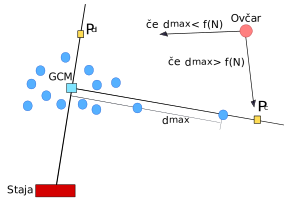
\includegraphics[width=0.8\textwidth]{../poglavja/images/zbiranje.pdf}
	\caption[Stanje zbiranja in vodenja črede]{Ovčar v stanju zbiranja ovc v čredo ali v stanju vodenja črede proti staji.} % narejena je s programom Inkscape
	\label{fig:zbiranje}
\end{figure}

\subsubsection{Stanje vodenja črede}

Ko ni nobena ovca več kot $f(N)$ oddaljena od GCM, se ovčar želi postaviti tako, da je čreda oziroma GCM med njim in stajo. Pri tem se postavi $f(N)$ stran od GCM, kot si lahko ogledamo na sliki~\ref{fig:zbiranje}. Točko označimo kot $P_d$.

\subsubsection{Ignoriranje dela črede}

Včasih pa se ovčar znajde v brezizhodni situaciji, ko sam ne obvladuje celotne črede. Zato smo naredili mejo za preklop med zbiranjem in vodenjem bolj ohlapno. Če imamo eno samo pobeglo ovco, je včasih nima smisla pripeljati bliže čredi, ker bi hitreje ostalo čredo privedel do staje in naknadno vanjo pripeljali tudi to ovco. Ovčar se zato odloči za vodenje črede že v primeru, ko je dovolj velik del črede največ $f(N)$ oddaljen od GCM. Dovoljeni delež pa se spreminja glede na število ovčarjev na sledeč način:
\begin{align}
p = p_z / n_s^{\sigma_s}, \label{eq:ignoriranje}
\end{align}
kjer je $p_z$ utež doslednosti zbiranja, $n_s$ število ovčarjev in $\sigma_s$ moč vpliva velikosti skupine ovčarjev. Več kot je ovčarjev, manj ignoriranih ovc dopuščamo, saj je večja skupina tudi dosti bolj sposobna zbrati veliko čredo. S tem se želimo izogniti možnosti, da bi ovčar ves čas le zbiral čredo, ki bi se mu razpršila vsakič, ko bi šel po ovco, ki jo je izbral, da jo mora pripeljati v čredo.

Pri tem je težava predvsem, da se GCM ne prilagaja vodenemu delu ovc ampak vsem ovcam in se tako lahko prestavi celo tako daleč od črede, da je ovčar ne more več voditi, saj njegove grožnje ne čuti dovolj velik del črede. A to se ne zgodi tako pogosto, sploh pa ne v primeru več ovčarjev, ko je delež ignoriranih ovc tako majhen, da GCM ne premakne dovolj na račun pobeglih ovc.

\subsubsection{Stanje naključnega premika}

Za primere, ko ovčar ovce pritisne v kot ograde ali pa se pojavi v kakšni drugi ravnovesni situaciji, ki ne dopušča uspeha, smo ovčarju dodali stanje naključnega premika, kjer si ovčar na vsakih $t_d + U(t_s)$ časovnih enot, kjer je $t_d$ deterministični del in $U(t_s)$ naključni dodatek enakomerno porazdeljen na intervalu $\lbrack 0, t_s\rbrack$, izbere naključno točko na pašniku, proti kateri se premika $t_p$ časovnih enot.

\subsubsection{Stanje premika za čredo}

Ker pa se še vedno lahko zgodi, da se ovčar postavi bliže staji kot GCM, se ovčar v takem primeru premika proti svojemu cilju glede na stanje zbiranja ali vodenja na prilagojen način.

Smer premika izračunamo kot
\begin{align}
s = \sqrt{\Vert S_i - F\Vert}(S_i - F) + (P - S_i) \sigma_n, \label{eq:zadaj}
\end{align}
kjer je $S_i - F$ vektor od staje proti ovčarju, $P - S_i$ vektor od ovčarja proti točki $P_d$ ali $P_c$, odvisno od zadoščenega pogoja za vodenje ali zbiranje, in $\sigma_n$ utež gibanja nazaj za čredo. V primeru, da je ovčar od staje dlje kot GCM, pa se giblje v smeri vektorja od njega proti izbrani točki glede na stanje.

\begin{figure}[ht]  % ali t za na vrhu ali h! za točno tukaj
	\centering
	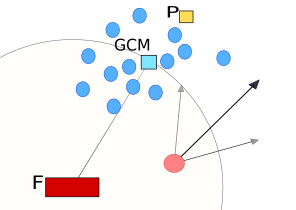
\includegraphics[width=0.49\textwidth]{../poglavja/images/zadaj.pdf}
	\caption[Stanje premika za čredo]{Ovčar v stanju premika za čredo.} % narejena je s programom Inkscape
	\label{fig:zadaj}
\end{figure}

\subsubsection{Izbira hitrosti gibanja}

Ovčar ima dve hitrosti med katerima gladko prehaja. Ovčar ima hitrost vodenja $v_{min}$, kadar je od točke $P_d$ ali $P_c$ oddaljen največ $d_t$ in kadar je od njega najbližja ovca oddaljena največ $d_0$. Sicer se giblje s hitrostjo $v_{max}$. S tem ovčar upočasni v bližini ovc in črede, ker bi jih sicer razkropil, če bi se jim preveč približal.

\subsection{Sodelovanje skupine ovčarjev}\label{sodelovanje}

Ovčar sam pogosto ne more zbrati črede ali pa je pri tem delu zelo neučinkovit zaradi odsotnosti grožnje, ko gre po pobegle ovce. Tedaj bi bilo dobro, da bi bilo psov več, da si pomagajo in delijo delo. Če ovčarji ne sodelujejo, bodo vedno želeli voditi isto ovco in učinka ne bo. Iščemo način, kako med ovčarje razdeliti delo.

Avtorici članka~\cite{aiba2020suggestion} sta primerjali štiri različne modele sodelovanja dveh psov ovčarjev. Pri tem se modeli razlikujejo v deljenju dela. V prvem modelu je en ovčar ves čas v stanju vodenja in eden v stanju zbiranja, v drugem modelu si vlogi izmenjujeta in nimata nikoli iste vloge, v tretjem največ en ovčar zbira čredo in v četrtem modelu preklapljata med stanjema neodvisno. Pri vseh modelih razen pri prvem si ovčarja čredo delita po premici skozi stajo in skozi GCM. Pri tem se je najbolje izkazal model, kjer sta ovčarja med stanjema neodvisno preklapljala.

Druga možnost poleg deljenja črede pa bi bila tudi iskanje optimalnih točk, kamor se morajo postaviti ovčarji in iskanje optimalne poti do teh točk. S tema problemoma se ukvarjajo avtorji člankov~\cite{lien2005shepherding, pierson2017controlling, pierson2015bio, lee2017autonomous}. Mi se bomo pri našem delu osredotočili na delitev črede. Ker pa si želimo vodenja z večjo skupino psov, moramo najti tudi primerno razdelitev črede na več enot.

Čredo bomo delili na Voronoieve celice z ovčarji v središčih. To pomeni, da ima vsak ovčar svojo Voronoievo celico in v njej vse tiste ovce, ki jim je najbližje izmed vseh ovčarjev. S tem bo vsaka ovca odgovornost le enega ovčarja in ko bo šel ovčar od črede daleč proč po neko ovco, si bodo ostali ovčarji razdelili ostalo čredo. Na sliki~\ref{fig:voronoi} si lahko ogledamo razdelitev črede in dela, kot je opisano v poglavju~\ref{zbiranje}.

\begin{figure}[ht]  % ali t za na vrhu ali h! za točno tukaj
	\centering
	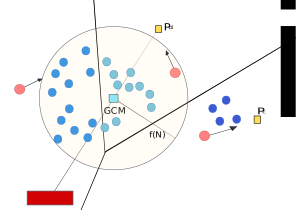
\includegraphics[width=0.9\textwidth]{../poglavja/images/voronoi.pdf}
	\caption[Razdelitev črede in nalog]{Razdelitev črede med tri ovčarje. Dva ovčarja sta v stanju vodenja in en je v stanju zbiranja.} % narejena je s programom Inkscape
	\label{fig:voronoi}
\end{figure}

Ovčarji želijo med seboj ohranjati neko minimalno udobno razdaljo. V ta namen smo med njimi dodali silo odboja z velikostjo $d_s / (\Vert r_{ij}\Vert + 1)$ v smeri od $j$-tega do $i$-tega ovčarja, ki ga močneje odbija od ovčarjev, ki so mu bliže, kjer je $d_s$ udobna razdalja med ovčarjema in $r_{ij}$ dejanska razdalja med njima. Ker pa ne želimo, da bi se ovčarjem poti križale in želimo njihove poti postaviti bolj vzporedno kot zaporedno, izračunamo tudi kot med njegovo smerjo in lokacijo drugega psa. Njegovi smeri dodamo silo v smeri stran od drugega ovčarja veliko $max(0, sin(\omega)) \sigma_o / (\Vert r_{ij}\Vert + 1)$, kjer je $\omega$ kot, pod kakršnim gre ovčar proti drugemu ovčarju in je $\sigma_o$ pomen smeri drugih ovčarjev.

\subsection{Premik ovčarja}

Ovčar se torej po zgoraj opisanem načinu giblje glede na stanje obnašanja in hitrost, pri čemer se giblje proti točki trenutnega cilja. Svojo smer pri tem prilagodi glede na prisotnost drugih ovčarjev. Na koncu pa njegovo smer še nekoliko popravimo. Dodamo ji šum tako, da jo zasukamo za naključen kot z intervala $\lbrack -e\pi/3, e\pi/3\rbrack$, kjer je $e$ relativna moč šuma. Nato njegovo smer zasukamo za kot $\nu$ stran od ograje, če je tej bliže kot 5~m in se giblje proti njej, okrog ovce, če je tej bliže kot $d_a$ ter okrog črede v primeru, da ovčar pride središču črede bliže od $\xi$ deleža razdalje med središčem črede in točko $P$ ($P_c$ ali $P_d$). Vse tri primere kroženja si lahko ogledamo na sliki~\ref{fig:zaokrozi}. Nato smer zgladimo glede na smer v prejšnjem časovnem koraku. S tem se ovčar giblje bolj naravno.

\begin{figure}[ht]  % ali t za na vrhu ali h! za točno tukaj
	\centering
	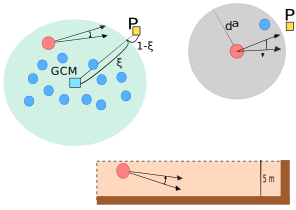
\includegraphics[width=0.9\textwidth]{../poglavja/images/zaokrozi.pdf}
	\caption[Izogibanje ograji, zaokrožanje okrog ovce in okrog črede]{Ovčar zaokroži blizu ograje, ovce ali črede.} % narejena je s programom Inkscape
	\label{fig:zaokrozi}
\end{figure}

V tabeli~\ref{table:ovcar} si lahko ogledamo uporabljene vrednosti parametrov in njihove meje za ostala dva modela.

\begin{table}[ht]
	\begin{center}
		\begin{tabular}{ c|l|c|c }
			\hline
			\textbf{Oznaka} & \textbf{Opis parametra} & \textbf{Vrednost} & \textbf{Interval} \\ \hline  
			$v_{max}$ & Najvišja hitrost & 7,5~m/s & - \\
			$v_{min}$ & Hitrost v stanju vodenja & 5~m/s & $\lbrack 0, v_{max} \rbrack$ \\
			$r_a$ & Faktor za dovoljeno velikost črede & 2~m & $\lbrack 0, 5 \rbrack$ \\
			$d_c$ & Razdalja za zbiranje & 10~m & $\lbrack 0, 30 \rbrack$ \\
			$d_a$ & Razdalja za zaznavo ovc na poti & 20~m & $\lbrack 0, 60 \rbrack$ \\
			$d_0$ & Razdalja za upočasnitve v bližini ovc & 10~m & $\lbrack 0, 30 \rbrack$ \\
			$d_f$ & Razdalja za upočasnitev v bližini cilja & 5~m & $\lbrack 0, 30 \rbrack$ \\
			$e$ & Relativna moč šuma & 30 \% & $\lbrack 0, 50 \rbrack$ \\
			$t_p$ & Trajanje naključnega premika & 3~s & $\lbrack 0, 10 \rbrack$ \\
			$t_d$ & Fiksen čas do naključnega premika & 60~s & $\lbrack 0, 90 \rbrack$ \\
			$t_s$ & Razpon naključnega dodatnega časa & 20~s & $\lbrack 0, 30 \rbrack$ \\
			$\sigma_r$ & Pomen oddaljenosti pobegle ovce od črede & 2 & $\lbrack -1, 4 \rbrack$ \\
			$\sigma_d$ & Pomen oddaljenosti pobegle ovce od ovčarja & 1 & $\lbrack -1, 4 \rbrack$ \\
			$d_b$ & Ovčar bližje cilju kot čreda & 2~m & $\lbrack -5, 50 \rbrack$ \\
			$p_z$ & Največji delež ignoriranih ovc & 15 \% & $\lbrack 0, 40 \rbrack$ \\
			$\sigma_s$ & Vpliv števila ovčarjev na delež ignoriranih ovc & 2 & $\lbrack -1, 4 \rbrack$ \\
			$\sigma_n$ & Odpor pred stanjem bližje cilju kot točka & 2 & $\lbrack 0, 20 \rbrack$ \\
			$d_s$ & Udobna razdalja med ovčarji & 20~m & $\lbrack 0, 40 \rbrack$ \\
			$d_t$ & Razdalja za upočasnitev v bližini točke & 12~m & $\lbrack 0, 20 \rbrack$ \\
			$\xi$ & Odpor pred stanjem pred točko & 95 \% & $\lbrack 0, 1 \rbrack$ \\
			$\nu$ & Zaokroževanje blizu ovc & $\pi / 6$ rad/s & $\lbrack 0, 2 \rbrack$ \\
			$\sigma_o$ & Pomen smeri drugih ovčarjev & 0,1 & $\lbrack -1, 1 \rbrack$ \\
			\hline
		\end{tabular}
	\end{center}
	\caption[Parametri vodenja psa ovčarja]{Parametri psa ovčarja, njihove uporabljene vrednosti za ročno razviti model in njihove meje za ostala dva modela gibanja psa ovčarja. Moje so v istih enotah kot izbrane vrednosti.}
	\label{table:ovcar}
\end{table}

\section{Model vodenja razvit z genetskim algoritmom} \label{genetski}

Če je ovčar čredi preblizu, se ovce razkropijo, če pa je predaleč jih ta ne more voditi. Najboljša razdalja pa je odvisna od števila ovc. Prav tako bi lahko našli boljše vrednosti tudi drugih parametrov modela (tabela~\ref{table:ovcar}) v odvisnosti od števila ovc, ovčarjev in modela gibanja ovc.

Ker je ročno razviti model pogosto neuspešen, si želimo najti optimalne vrednosti parametrov. Za vsak parameter lahko postavimo neke smiselne meje, kjer bi ta vrednost lahko bila. Ampak dobljeni prostor (produkt 21 intervalov, največja hitrost je konstantna) je prevelik, zato moramo najti nek način iskanja najboljših vrednosti v tem prostoru. Četudi bi zvezne intervale razdelili na le 10 diskretnih vrednosti, bi tako morali preveriti $10^{21}$ kombinacij vrednosti parametrov. Če bi algoritem le vrnil ničelni izhod, bi en računalnik s 16 jedri in hitrostjo procesorja 3,5 GHz preverjal vse kombinacije več kot 580 let. Torej nam tu ne bi pomagala niti uporaba več računalnikov, saj nikakor ne bi zaključili vseh dosti bolj kompleksnih simulacij v nekem doglednem času.

Odločili smo se za pristop z genetskim algoritmom za optimizacijo parametrov, ki temelji na ideji naravne selekcije, kar poznamo iz evolucije. Ker je algoritem vseeno zamuden, smo simulacijo omejili na 3 minute (omejeno z številom korakov simulacije, ki ustrezajo 3 minutam in ne z dejanskim časom izvajanja) in jo nato prekinili, če se simulacija še ni sama zaključila z uspešnim izidom. Genetski algoritmi so populacijski algoritmi za optimizacijske probleme. Pri implementaciji smo se zgledovali po podrobni razlagi algoritma v~\cite{natureOfCode}.

Ideja genetskih algoritmov je ta, da imamo začetno populacijo naključnih genov, tej začetni generaciji pa sledijo generacije, ki naj bi bile sčasoma v povprečju vedno boljše. Pri tem moramo dobro definirati, kaj je gen in kaj pomeni, da je nek gen "boljši".

\subsection{Gen in evalvacija uspešnosti gena}

Vsak osebek v populaciji ima določene vrednosti vseh 21 parametrov in temu zaporedju števil pravimo gen. Tako je na primer genotip za hitrost ovčarja v stanju vodenja pri ročno razvitem modelu enak 2/3 (le numerična vrednost), fenotip pa je njegova izražena hitrost v stanju vodenja 5 m/s. Opazimo, da se med evolucijo lahko pojavi tudi gen, ki ustreza fenotipu ročno razvitega ovčarja. Torej lahko pričakujemo ob koncu evolucije vsaj tako dober gen ali celo boljšega in s tem večjo uspešnost vodenja, saj bi tudi ročno razviti model izumrl, če ni vsaj primerljiv z najboljšim genom.

Da evolucija deluje, mora biti v začetnem genomu dovolj različnih genov. Če geni niso dovolj različni, bodo naslednje generacije preveč podobne prvi in odvisne od začetka simulacije. Če pa genov ni dovolj, se lahko hitro izgubi potencial, ki se skriva v posameznem genu, a ta prehitro izumre.

Uspešnost posameznega gena pa moramo nekako oceniti, da jih potem lahko primerjamo. Za to potrebujemo funkcijo uspešnosti za evalvacijo gena. Pri tem upoštevamo čas potreben za simulacijo (zadnja ovca v staji), število ovc na pašniku ob koncu simulacije, oddaljenost preostanka črede od staje in čase prihodov v stajo za vse ovce v staji. Funkcija naj bi bila konveksna v primeru, ko je pomembna dejanska ocenjena vrednost in ne le razvrstitev med ostalimi geni.

Naša izbrana funkcija za oceno uspešnosti posamezne simulacije je
\begin{align}
\phi(N, (t_j)_{j_1}^k, GCM) &= 210\Big(\frac{t_{MAX} - t_N}{t_{MAX}}\Big)^2\frac{1}{N}\sum_{j=1}^k \frac{t_{MAX} - t_j}{t_{MAX}} \label{eq:genetski} \\
 &+ \frac{1}{1 + N - k + (N - k)\Vert GCM - F\Vert}, \nonumber
\end{align}
kjer je $t_{MAX}$ časovna omejitev simulacije v sekundah, $N$ začetno število ovc, $k$ število ovc pripeljanih v stajo in $F$ lokacija staje. Po tej formuli dobimo večjo uspešnost za simulacije, ki prej v stajo pripeljejo večji delež črede. Tako je bolj uspešen gen, kjer je zadnja ovca prej v staji. Nekoliko manj pomembno je, da so bile ovce v povprečju prej pripeljane v stajo oziroma, da nam je ostal večji delež časa. Faktor 210 služi le normalizaciji, da je želena uspešnost med 0 in 100. Ker pa je v primeru $t_N = t_{MAX}$, ko je na pašniku še vsaj ena ovca, prvi člen enak 0, mu prištejemo še drugi člen, kjer je pomembno število preostalih ovc na travniku in je še nekoliko manj pomembna razdalja med GCM in F. S tem lahko po uspešnosti razvrstimo tudi simulacije, kjer je na pašniku ostala še vsaj ena ovca.

\subsection{Nova generacija}

Ko ocenimo uspešnost vseh genov v generaciji, moramo narediti novo generacijo, kjer damo večjo verjetnost za ponovno pojavitev genom, ki jim je šlo bolje. Pri tem pa moramo ohranjati dovoljšnjo variabilnost genoma.

Genetski algoritem sestoji iz več generacij. Novo generacijo pa naredimo iz prejšnje z uporabo večje verjetnosti parjenja za uspešnejše gene, križanja obeh genov iz para in mutacij na dobljenem genu. Oglejmo si podrobnosti teh korakov. Na sliki~\ref{fig:genetski} pa lahko vidimo grafični prikaz razmnoževanja.

\begin{figure}[ht]  % ali t za na vrhu ali h! za točno tukaj
	\centering
	\includegraphics[width=0.9\textwidth]{../poglavja/images/genetski.pdf}
	\caption[Razmnoževanje uspešnejših genov]{Najprej geni z uspešnostjo (vhod), več ponovitev v bazenu bolj uspešnim, parjenje, križanje, mutacije (izhod)} % narejena je s programom Inkscape
	\label{fig:genetski}
\end{figure}

\subsubsection{Parjenje} \label{parjenje}

Obstaja mnogo različnih načinov parjenja. Lahko določimo koliko najboljših genov se bo z enako verjetnostjo razmnoževalo, čemur rečemo elitna metoda, a tu se del genov ne pojavlja več v naslednjih generacijah razen v primeru mutacij. Mi pa smo si izbrali verjetnostni pristop, kjer ima vsak gen verjetnost parjenja odvisno od uspešnosti.

Za ta namen pripravimo bazen genov, iz katerega kasneje dobimo naključne pare. Pri tem v bazen postavimo $round(2 i^2 / n)$ kopij gena z $i$-to najnižjo uspešnostjo, če imamo do konca evolucije še vsaj tri generacije, kjer je $n$ velikost populacije v eni generaciji. V zadnjih treh generacijah smo v bazen postavili $round(2 i^3 / n)$ kopij $i$-tega gena, s čimer smo naredili še večji pritisk na naravno selekcijo, saj imajo slabši posamezniki še manjše možnosti za parjenje, s čimer je pristop na nek način bolj podoben elitni metodi. Na sliki~\ref{fig:verjetnost-parjenja} si lahko ogledamo verjetnosti za parjenje v seznamu genov razvrščenem po uspešnosti.

\begin{figure}[ht]  % ali t za na vrhu ali h! za točno tukaj
	\centering
	\includegraphics[width=0.5\textwidth]{../poglavja/images/parjenje.pdf}
	\caption[Verjetnost parjenja]{Graf z obema krivuljama} % narejena je s programom Inkscape
	\label{fig:verjetnost-parjenja}
\end{figure}

Iz dobljenega bazena vzamemo $n$ parov genov, pri čemer je edini pogoj, da oba starša tega para nista isti posameznik.

\subsubsection{Križanje}

Vsak par kromosomov naključno križamo in s tem dobimo večjo variabilnost genov v populaciji. Uveljavljenih je več pristopov križanja. Ker želimo ohranjati dolžino gena se osredotočimo le na rezanje obeh genov v istih točkah in na uniformno izbiro. Križanje z rezanjem pomeni, da v eni ali dveh točkah prerežemo oba gena in nato vrnemo gen, kjer se izmenjujejo kosi, ki prihajajo od obeh staršev. Ker pa sosednost znotraj gena nič ne pomeni, smo se odločili za uniformno križanje, kjer naključno vsako vrednost iz zaporedja v nov gen kopiramo od enega ali drugega izmed staršev. Tako se gena enakomerno premešata.

\subsubsection{Mutacija}

Da ohranjamo raznolikost genoma in se s tem izogibamo lokalnim optimumom, dobljenemu genu na vsakem mestu z verjetnostjo $p$ vrednost izberemo naključno z intervala dopustnega za to vrednost. Pri tem smo v vsakem koraku naredili ožji interval, s katerega smo vrnili naključno vrednost. S tem smo sčasoma dovoljevali le še manjše spremembe, saj preveč mutacij lahko onemogoča evolucijski napredek skozi generacije. Vrnemo naključno vrednost z intervala $\lbrack x - \frac{1}{generacija} (M - m), x + \frac{1}{generacija} (M - m)\rbrack \cap \lbrack m, M \rbrack$, kjer je $x$ vrednost po križanju, $M$ zgornja meja izbranega parametra, $m$ spodnja meja izbranega parametra in $generacija$ zaporedna številka generacije. Meje parametrov lahko najdemo v tabeli~\ref{table:ovcar}.

\subsubsection{Državno tekmovanje}

Pri istem genu pa so ovčarji lahko različno uspešni. Želimo se izogniti izbiri gena, ki je imel le \textit{srečo} in v povprečju ni tako dober, prav tako želimo zmanjšati verjetnost neuspeha. V ta namen smo uvedli drugačno točkovanje v zadnjih treh generacijah. Do te točke so slabi geni večinoma že izumrli, saj je verjetnost, da ima slab gen čez veliko generacij še potomce, ki so mu podobni, vedno manjša. Celo v povprečju mu mora iti dobro, sicer najverjetneje do konca evolucije niti ne pride. Na koncu pa imamo že zelo uspešne gene, med katerimi si želimo vzeti najzanesljivejšega. Med zadnjimi tremi poostrimo vrednotenje, da onemogočimo uspeh na podlagi \textit{sreče}. Temu pristopu bomo rekli \textit{državno tekmovanje}. Prav tako bomo poleg drugačne funkcije uspešnosti uporabljali tudi bolj elitno parjenje, kot smo za zadnje tri generacije že omenili v poglavju~\ref{parjenje}.

Novo točkovanje temelji na treh evalvacijah istega gena z enako funkcijo uspešnosti kot prej po formuli~\eqref{eq:genetski}. Za vsak gen dobljene tri uspešnosti $f_1, f_2, f_3$ združimo v 
\begin{align}
\Phi(f_1, f_2, f_3) &=\frac{\sum_{i\in\lbrack 3\rbrack} f_i}{3}~ min_{i\in\lbrack 3\rbrack} f_i, \label{eq:drzavno}
\end{align}
kjer z $\lbrack 3\rbrack$ označujemo množico naravnih števil do vključno 3. Gen je torej boljši, če je v povprečju uspešnejši in če je njegova najnižja uspešnost dovolj visoka.

\subsection{Naša implementacija genetskega algoritma}

Z genskim algoritmom smo iskali najboljši gen za določeno število psov ovčarjev, določeno začetno število ovc in model gibanja ovc. Velikosti črede, za katere smo iskali najboljši gen, so 5, 10, 25, 50, 75 in 100. Ovčarjev pa je bilo 1, 2, 3 ali 4. Za ostale velikosti črede ali število psov lahko posplošimo tako, da vzamemo najbolj podobno število ovc in psov. Tako smo našli dobre gene za 72 začetnih kombinacij.

Vrednosti parametrov genetskega algoritma si lahko ogledamo v tabeli~\ref{table:genetski}. Skico naše implementacije z državnim tekmovanjem pa lahko vidimo v algoritmu~\ref{alg:genetski}.

\begin{table}[ht]
	\begin{center}
		\begin{tabular}{ c|l|c }
			\hline
			\textbf{Oznaka} & \textbf{Opis parametra} & \textbf{Uporabljena vrednost} \\ \hline  
			$n$ & Velikost populacije & 40 \\ 
			$G$ & Število generacij & 27 \\
			$p$ & Verjetnost mutacije & 1 \% \\
			$t_{MAX}$ & Največji čas simulacije & 180~s \\
			\hline
		\end{tabular}
	\end{center}
	\caption[Parametri genetskega algoritma]{Parametri genetskega algoritma.}
	\label{table:genetski}
\end{table}

\begin{algorithm}
	\caption{Genetski algoritem} 
	\begin{algorithmic}[1]
		\State Inicializacija()
		\State Evalvacija()
		\For {$generacija=1,2,\ldots,G$}
			\State Razmnoževanje()
			\State Križanje()
			\State Mutacija()
			\If{$generacija \leq G-3$}
				\State Evalvacija()
			\Else
				\State 3x Evalvacija()
			\EndIf
		\EndFor
	\end{algorithmic} 
	\label{alg:genetski}
\end{algorithm}

\section{Model vodenja z adaptivnim genom}

Problem se pri genetskem algoritmu lahko pojavi, ko se število ovc na pašniku močno zmanjša, saj so parametri ves čas enaki, odvisni le od začetnega števila ovc. Parametre želimo prilagajati trenutnemu stanju na pašniku, številu ovc, psov in še čemu, kar bi lahko koristilo uspešnosti vodenja črede. Celo bolje bi bilo, če bi se ovčarji lahko naučili česa novega, izvirnega, česar naš model ne predvideva niti ob spreminjanju parametrov. Želimo mu dati čim bolj proste roke pri izbiri smeri in hitrosti.

Za to bomo uporabili metode umetne inteligence, ki nam omogočajo učenje čim boljših potez v določenem trenutku. Z vodenjem črede s pomočjo spodbujevanega učenja so se ukvarjali tudi avtorji člankov~\cite{obstacles} in~\cite{sarsa}. Ker je naš program pripravljen v programu Unity, smo se odločili za uporabo paketa ML Agents, ki temelji na spodbujevanem učenju, konkretno na PPO algoritmu. V tem poglavju bomo predstavili ta izbrani algoritem.

\subsection{Spodbujevano učenje}

Spodbujevano učenje je osredotočeno na interakcijo med agentom in okoljem, pri čemer agent maksimizira nagrade, ki jih dobi iz okolja, ko v danem stanju naredi neko potezo~\cite{reinforcement}, kot lahko vidimo na sliki~\ref{fig:reinforcement}. Agent je hkrati učenec in odločevalec. Tekom učenja skrbi za ravnotežje med raziskovanjem nepoznanega in izkoriščanjem pridobljenega znanja.

\begin{figure}[ht]  % ali t za na vrhu ali h! za točno tukaj
	\centering
	\includegraphics[width=0.7\textwidth]{../poglavja/images/reinforcement.pdf}
	\caption[Agent in okolje pri spodbujevanem učenju]{Interakcije med agentom in okoljem.} % narejena je s programom Inkscape
	\label{fig:reinforcement}
\end{figure}

Model sicer pogosto temelji na markovskem procesu odločanja, za katerega bi lahko narisali graf stanj in povezav med stanji z verjetnostmi prehodov, ampak za algoritme spodbujevanega učenja ne potrebujemo poznavanja tega grafa, saj ga algoritem sam raziskuje in se uči najboljših odločitev v raziskanem prostoru brez računanja in pomnjenja samega grafa.

Okolje modela je določeno s stanji $s \in S$, potezami $a\in A(s)$, ki so agentu na voljo v stanju $s$, pripisanimi numeričnimi nagradami $r(s, s^\prime, a) \in R$ ob izbrani potezi $a$ in spremembi stanja iz $s$ v stanje $s^\prime$ ter verjetnostmi stanj $P(s^\prime \vert s, a)$ doseženih iz stanja $s^\prime$ z uporabo poteze $a$. Prav ta verjetnost in vrednosti nagrad so nam običajno neznane.

Agent se med možnimi potezami odloča na podlagi svoje strategije izbire akcij. Med učenjem posodablja strategijo $\pi(a, s)=P(a\vert s)$, ki predstavlja verjetnost izbire poteze $a$ v stanju $s$ tako, da je pričakovana vsota nagrad v prihodnosti največja, torej maksimiziramo vrednostno funkcijo izbranega stanja $s$ ob uporabi izbrane strategije
\begin{align}
V^\pi(s) &= E\lbrack r_{t+1} + \gamma r_{t+2} + \gamma^2r_{t+3} + \ldots\vert s_t=s, \pi\rbrack, \label{eq:value}
\end{align}
kjer sledimo trenutni strategiji $\pi$ in je $\gamma\in\lbrack 0, 1)$ diskontni faktor, ki uravnoteži pomen trenutne nagrade in prihodnjih. Funkcija $V(s)$ oceni dolgoročni obet uporabe strategije $\pi$ iz trenutnega stanja, pri čemer da manjšo težo oddaljenim nagradam. Tako se agent načeloma izogiba potezam, ki mu bodo dolgoročno škodovale in se raje odloča za tiste, ki mu obljubljajo večjo nagrado v krajšem času. Pri učenju pa je pomembno, da agent tudi raziskuje po prostoru stanj. K temu ga spodbudimo z naključnimi potezami z verjetnostjo $\epsilon$. Ta parameter je običajno najprej nastavljen na neko začetno vrednost med 0 in 1, potem pa pada skozi čas proti 0. S tem agent najprej predvsem raziskuje, potem pa vedno bolj izkorišča svoje znanje, ki si ga je pridobil. Vseeno pa se lahko ujame v lokalnem optimumu.

Agent mora oceniti lastnosti okolja, predvsem verjetnost prehodov med stanji $P(s^\prime\vert s, a)$, da lahko oceni vrednosti stanj. Na principu spodbujevanega učenja z nagradami in kaznimi se v veliki meri učijo tudi človeški možgani. Razvitih je že mnogo algoritmov za učenje optimalne strategije, kot so TD-Learning, Q-Learning, SARSA, globoko Q-učenje, PPO in drugi. Paket ML Agents uporablja algoritem PPO, zato si tega nekoliko podrobneje oglejmo.

\subsubsection{Optimizacija z bližnjo strategijo}

Motivacija za optimizacijo z bližnjo strategijo (Proximal Policy Optimization - PPO) je vprašanje, kako kar najbolj izboljšati strategijo na podlagi trenutne, brez da bi zaradi slučajne velike nagrade pomotoma stopili predaleč in povzročili nenaden padec uspešnosti strategije. PPO za vrednosti parametrov nima omejitev, ampak ima omejitev le na velikosti koraka, s katerim spremenimo parametre. Omejitev je postavljena z namenom, da je nova strategija dovolj podobna prejšnji, saj bolj zaupamo vrednostim parametrov blizu prejšnje strategije, ker nočemo uničiti naučenega na podlagi posamezne ocene.

PPO je algoritem, ki se uči napovedovanja pričakovanih nagrad, da se tako odloča za najbolj obetavne poteze v danem stanju. S pomočjo gradientnega spusta spreminjamo vektor parametrov $\theta_k$ in s tem strategijo $\pi^{\theta_k}$, ki je odvisna od tega vektorja. Vektor parametrov si lahko predstavljamo kot vektor uteži v nevronski mreži. Pri tem moramo stanje in potezo nekako numerično predstaviti modelu. Poleg nevronske mreže, ki izračuna verjetnost neke poteze na podlagi stanja, definiramo tudi vrednostno funkcijo $\hat{V}^{\phi_k}(s)$, ki oceni vrednost prihodnjih nagrad z uporabo nevronske mreže, ki jo naučimo ocenjevati pričakovane nagrade na podlagi stanja. Tudi ta funkcija mora biti odvedljiva in odvisna od vektorja parametrov $\phi_k$. 

PPO je za razliko od Q-Learning in nekaterih drugih algoritmov spodbujevanega učenja primeren tudi za zvezna prostora možnih potez in stanj. Razvil ga je Schulman iz OpenAI s sodelavci. Predstavljen je v članku~\cite{ppo-clanek}. Algoritem je po rezultatih primerljiv drugimi trenutno najboljšimi algoritmi spodbujevanega učenja, njegova prednost pa je predvsem v relativno enostavni implementaciji in nastavljanju parametrov algoritma.

Pri tem algoritmu definiramo tudi primerjalno funkcijo
\begin{align}
L(s,a,\theta_k,\theta) = \min\left(\frac{\pi_{\theta}(a|s)}{\pi_{\theta_k}(a|s)}  A_t^k(s,a),~g(\epsilon, A_t^k(s,a))\right), \label{eq:lclip}
\end{align}
kjer je $\theta_k$ trenutni vektor parametrov strategije (v našem primeru uteži nevronske mreže), $\theta$ izbrani vektor parametrov strategije, ki ga primerjamo s trenutno strategijo, $A_t^k$ je ocenjena donosnost poteze ob času $t$, $\epsilon$ je parameter, ki omejuje spremembo strategije, običajno med 0.1 in 0.2 ter
\begin{align}
g(\epsilon, A) = \Big\{
\begin{array}{ll}
(1 + \epsilon) A & A \geq 0 \\
(1 - \epsilon) A & A < 0.
\end{array}
\end{align}

Donosnost poteze je enaka $A_t^k = V(s_t) - \hat{V}^{\phi_k}(s_t)$. Torej predstavlja razliko med točno vrednostjo vrednostne funkcije izračunane na podlagi dejanskih nagrad, ki ni samo ocena in njeno oceno izračunano po formuli pridobljeni na podlagi preteklega znanja z vektorjem parametrov $\phi_k$, ki se jih prav tako sproti učimo za boljše ocenjevanje pričakovanih nagrad.

PPO posodablja strategijo na sledeč način:
\begin{align}
\theta_{k+1} = \arg \max_{\theta} \underset{s,a \sim \pi_{\theta_k}}{{\mathrm E}}\lbrack
L(s,a,\theta_k, \theta)\rbrack, \label{eq:posodobi}
\end{align}
običajno z več koraki stohastičnega gradientnega spusta za maksimizacijo primerjalne funkcije. Za lažjo optimizacijo je priporočljivo, da sta vrednostna funkcija in strategija odvedljivi. Če je donosnost poteze pozitivna, oziroma je višina nagrad nad pričakovanji, verjetnost izbire poteze $a$ pa je po strategiji $\pi_\theta$ večja kot prej, raje izberemo to strategijo, saj želimo verjetnost dobre poteze povečati. Prav tako zmanjšamo verjetnost slabe poteze. Funkciji $min$ in $g$ pa služita temu, da damo strategijam z relativno razliko med verjetnostjo izbire poteze $a$ v primerjavi s staro strategijo večjo od $\epsilon$ enako primerjalno vrednost. S tem se izognemo navduševanju nad velikimi vrednostmi primerjalne funkcije, ki bi nas potegnile daleč od trenutne strategije, ki ji dolgoročno bolj zaupamo, saj ni odvisna le od posamezne uspešnosti simulacije, ki je lahko le posledica šuma, ki ga povzroča velika variabilnost vrednosti nagrad. S tem se strategija ne more dramatično spremeniti, lahko pa se poveča vrednost vrednostne funkcije. V algoritmu~\ref{alg:ppo} si lahko postopek podrobneje ogledamo.

\begin{algorithm}[ht]
	\caption{PPO}
	\label{alg:ppo}
	\begin{algorithmic}[1]
		\State Vhod: začetni parametri strategije $\theta_0$, začetni parametri vrednostne funkcije $\phi_0$
		\For{$k = 0,1,2,...$}
		\State Zberi množico izvedenih simulacij ${\mathcal D}_k$ z uporabo strategije $\pi_{\theta_{k}}$.
		\State Izračunaj dobljene nagrade $(r_t)_{t=0}^T$ za vsako simulacijo.
		\State Izračunaj ocene donosnosti $(A_t^k)_{t=0}^T$ temelječ na vrednostni funkciji $\hat{V}_{\phi_{k}}$.
		\State Posodobi strategijo s pomočjo primerjalne funkcije:
		\begin{equation*}
		\theta_{k+1} = \arg \max_{\theta} \frac{1}{|{\mathcal D}_k| T} \sum_{\tau \in {\mathcal D}_k} \sum_{t=0}^T L(s_t, a_t, \theta_k, \theta),
		\end{equation*}
		običajno preko stohastičnega gradientnega spusta.
		\State Popravi vrednostno funkcijo z regresijo, da bo čim manjša napaka vsote kvadratov:
		\begin{equation*}
		\phi_{k+1} = \arg \min_{\phi} \frac{1}{|{\mathcal D}_k| T} \sum_{\tau \in {\mathcal D}_k} \sum_{t=0}^T (V(s_t) - \hat{V}_\phi(s_t))^2,
		\end{equation*}
		običajno preko algoritma gradientnega spusta.
		\EndFor
	\end{algorithmic}
\end{algorithm}


\subsection{Adaptivni gen}

Pri učenju modela smo najprej poizkusili na način, da bi ovčarju dali proste roke, da se odloča o smeri in hitrosti na podlagi opazovanj. Poizkušali smo z različnimi funkcijami za nagrajevanje, veliko različnimi opazovanimi vrednostmi in celo z demonstracijami, kar pomeni, da smo algoritem najprej učili brez, da bi ta poskušal z naključnimi potezami, ampak s potezami, kakršne je izbiral ovčar z optimalnim genom iz genetskega modela. Če smo dali ovčarju popolnoma proste roke, se ni uspešno naučil niti sam, celo z eno samo ovco. Ta prostor stanj je bil prevelik, da bi ga agent uspešno spoznal in se iz njega česa naučil. Običajno se v različnih virih ML Agents uporablja za bolj enostavne probleme. Poizkusili smo še z manj svobodnim modelom. Ta model smo poimenovali \textit{adaptivni gen}.

Ideja je, da damo ovčarju le nekaj opazovanih vrednosti, on pa se odloči za najboljši gen znotraj dovoljenih meja za vsako vrednost v genu. Gen je definiran enako kot v poglavju~\ref{genetski}. Adaptivni gen bi moral imeti celo boljše rezultate kot optimalni gen iz genetskega algoritma, saj ima ta model še več svobode in vključuje tudi možnost, da se nauči enakih genov kot druga dva modela, če jih vmes ne spreminja. Vemo, da model naučen z genetskim algoritmom deluje, dovolj bi ga bilo le izboljšati. Ovčar naj se nauči izbire gena iz le nekaj osnovnih opazovanih lastnosti. Ker pa je učenje precej zamudno, smo se odločili le za Ginellijev model ovc in le za enega ovčarja na naključno veliki čredi med 1 in 10 ovcami, saj je ta model bolj podoben naravnemu obnašanju ovc, ovčar pa je imel probleme le sam, s sodelovanjem pa je model precej uspešen že z genom dobljenim z genetskim algoritmom. Večje črede pa se mu žal ni uspelo naučiti voditi niti v več urah.

\subsection{Naša implementacija modela}

Model se odloča vsakih 20 korakov, kar pomeni na 0,4~s. Med posameznimi odločitvami uporablja gen, ki ga je nazadnje izbral. Trajanje simulacije $T$ smo navzgor omejili na 750 izračunov gena (300~sekund oziroma 5~minut), kar je več kot tri minute z namenom, da se lahko uči vodenja tudi, če je za zbiranje potreboval več časa. Za primerni vrednosti parametrov modela sta se izkazali vrednosti $\epsilon=0,2$ in $\gamma=0,99$. Pred učenjem smo naredili 128 simulacij za pospešitev učenja na podlagi demonstracij. Za izbiro poteze se je model naučil uteži za nevronsko mrežo s 5 plastmi po 512 nevroni.

\subsubsection{Nagrajevanje}

Ovčar dobi nagrado veliko $\frac{1}{20T}$ vsakič, ko center črede (GCM) premakne staji bliže, kot je bil center blizu staji kadar koli pred tem znotraj simulacije. V vsakem časovnem koraku pa dobi prav tako kazen, ki ga spodbuja k hitrejšemu reševanju problema. Kar pomeni, da ovčar dobi kazen v primeru, da črede ne pripelje bliže staji, sicer ne dobi ničesar.

Ko spravi zadnjo ovco v stajo dobi še $4(\frac{T - t}{T})^2$ nagrade za uspešno opravljeno nalogo, kjer je $t$ čas ob zaključku simulacije. Z višino nagrade ga spodbujamo k hitrejšemu vodenju.

\subsubsection{Opazovanje vrednosti}

Stanje, v katerem je ovčar, definiramo s številom ovc na pašniku, deležem pobeglih ovc glede na trenutni delež dovoljenih pobeglih ovc, razliko med GCM in stajo ter ovčarjem in stajo v smeri $x$ in $z$. Uporabimo izračunane vrednosti v tem in prejšnjem koraku posodabljanja gena.

Poleg tega ovčar opazuje tudi oddaljenost objektov v smereh devetih žarkov razvrščenih okrog njega s skupnim kotom $120^\circ$. Pri tem lahko loči med ovco in ograjo oddaljeno največ 50~m. Na sliki~\ref{fig:zarki} si lahko ogledamo razvrstitev žarkov.

\begin{figure}[ht]  % ali t za na vrhu ali h! za točno tukaj
	\centering
	\includegraphics[width=0.8\textwidth]{../poglavja/images/zarki.png}
	\caption[Predstavitev prostora z žarki]{Predstavitev prostora z žarki. Ovčar lahko prepozna objekt in določi razdaljo do njega.} % narejena je s programom Inkscape
	\label{fig:zarki}
\end{figure}


\section{Program iOvčar IZIDOR}

Za učenje in testiranje modelov smo pripravili program, ki smo ga poimenovali \textit{iOvčar IZIDOR}. Program je napisan v programskem jeziku $C\#$, za vizualizacijo smo uporabljali program Unity in za spodbujevano učenje paket ML Agents\footnote{Pri učenju nam je bila v veliko pomoč spletna stran \url{https://www.immersivelimit.com} [ogled 9.\ 3.\ 2021].}. Program nam je omogočal grafični prikaz simulacije in beleženje rezultatov. Na slikah~\ref{fig:pasnik} in~\ref{fig:meni} si lahko ogledamo izgled simulacijskega okolja.

V programu so modeli vodenja psa ovčarja običajno poimenovani na drugačen način. Ročno razviti model je imenovan "Voronoi", model razvit z genetskim algoritmom je "AI1" in model z adaptivnim genom je "AI2".

\begin{figure}[ht]  % ali t za na vrhu ali h! za točno tukaj
	\centering
	\includegraphics[width=0.7\textwidth]{../poglavja/images/obicajen-pogled.png}
	\caption[Pogledi med simulacijo]{Običajen pogled med simulacijo. Program nam omogoča tudi pogled od zgoraj in izza izbranega ovčarja.} % narejena je s programom Inkscape
	\label{fig:pasnik}
\end{figure}

\begin{figure}[ht]  % ali t za na vrhu ali h! za točno tukaj
	\centering
	\includegraphics[width=0.8\textwidth]{../poglavja/images/meni.png}
	\caption[Meni programa]{Meni za izbiro nastavitev v programu.} % narejena je s programom Inkscape
	\label{fig:meni}
\end{figure}

\section{Rezultati}

V tem poglavju si bomo ogledali nekaj rezultatov uspešnosti različnih modelov. Za vsako kombinacijo števila ovčarjev, ovc, modela gibanja ovc in modela vodenja ovčarja smo naredili 100 simulacij.

\begin{figure}[H]  % ali t za na vrhu ali h! za točno tukaj
	\centering
	\includegraphics[width=\textwidth]{../poglavja/grafi/prezivetvena-Voronoi.png}
	\caption[Delež ovc na pašniku skozi čas]{Delež ovc na pašniku skozi čas za ročno razvit model vodenja ovc. Legenda je za vse grafe enaka in se nahaja le na desnem grafu v tretji vrstici. Vsak stolpec grafov prikazuje izbran model gibanja ovc, vrstica pa velikost črede (25, 50, 75 ali 100). Poleg krivulje za povprečen delež ovc na pašniku ob danem času je na grafu viden tudi interval zaupanja s stopnjo zaupanja 95~\%.} % narejena je s programom Inkscape
	\label{fig:prezivetvena}
\end{figure}

Na sliki~\ref{fig:prezivetvena} si lahko ogledamo povprečen delež ovc na pašniku ob določenem času do konca simulacije pri 180 sekundah pri vodenju psa z ročno razvitim modelom. Hitro opazimo, da so si rezultati pri Str{\"o}mbomovem in popravljenem Str{\"o}mbomovem modelu gibanja ovc zelo podobni. Ovčar je najuspešnejši pri Ginellijevem modelu. Več ovčarjev običajno pomeni večjo uspešnost. Pri tem je vpliv začetne razdalje najbližjega ovčarja do črede predvsem pri večjih čredah praktično zanemarljiv.

\subsection{Iskanje optimalnega gena}

Na slikah~\ref{fig:fit}--\ref{fig:Ge-gen2} si bomo ogledali, kako so se nekatere opazovane lastnosti spreminjale skozi generacije. Na vseh grafih temno modra krivulja predstavlja mediano vrednosti izbrane lastnosti, rdeči črti predstavljata ekstremne vrednosti, vmes pa je poleg mediane tudi temnejši moder pas, ki se razprostira od 15.\ do 85.\ percentila. Zelena črta predstavlja mediano vrednosti za ročno razviti model, oranžna črta pa predstavlja začetek državnega tekmovanja. V tem delu se bomo pri izrisovanju osredotočili le na Ginellijev in Str{\"o}mbomov model ovc.

Na sliki~\ref{fig:fit} vidimo gibanje ocenjene uspešnosti gena izračunane po formuli~\eqref{eq:genetski}, na sliki~\ref{fig:maxt} trajanje posamezne simulacije skozi generacije, na sliki~\ref{fig:uspeh} delež ovc v staji ob koncu simulacije, na sliki~\ref{fig:Ge-gen2} pa si lahko ogledamo gibanje genotipa za parameter $r_a$, ki predstavlja faktor za dovoljeno velikost črede.

Na nobeni izmed slik ni opaziti pozitivnega pomena državnega tekmovanja, saj so na državnem tekmovanju večinoma le še geni, ki imajo dovolj visoko povprečno in minimalno uspešnost. Poleg tega je v tej točki variabilnost genoma že zelo majhna.

\begin{figure}[H]  % ali t za na vrhu ali h! za točno tukaj
	\centering
	\includegraphics[height=0.4\textheight]{../poglavja/grafi/Ginelli-evolucija-Fitness.png}
	\includegraphics[height=0.4\textheight]{../poglavja/grafi/Stroembom-evolucija-Fitness.png}
	\caption[Uspešnost skozi generacije]{Uspešnost skozi generacije. Opazimo, da se praviloma hitro poveča. Pri tem je na koncu uspešnost običajno vsaj primerljiva z ročno razvitim modelom. Zelene črte pogosto ne vidimo, ker je več kot polovica simulacij v nekaterih primerih neuspešnih. Vodenje ovc po Ginellijevem modelu se zdi veliko lažje za naš model vodenja, saj se model hitro nauči dobrega gena za poljubno velikost črede ali število ovčarjev.} % narejena je s programom Inkscape
	\label{fig:fit}
\end{figure}

\begin{figure}[H]  % ali t za na vrhu ali h! za točno tukaj
\centering
\includegraphics[height=0.4\textheight]{../poglavja/grafi/Ginelli-evolucija-MaxT.png}
\includegraphics[height=0.4\textheight]{../poglavja/grafi/Stroembom-evolucija-MaxT.png}
\caption[Trajanje simulacije skozi generacije]{Trajanje simulacije skozi generacije. Rezultati so pričakovani glede na ocenjeno uspešnost na sliki~\ref{fig:fit}. Na večini grafov opazimo, da je mediana na koncu blizu minimalnega časa. Trajanje simulacije je navzdol omejeno s hitrostjo črede. Hitrost teka je pri ovcah po obeh modelih enaka, ampak je čreda ovc po Str{\"o}mbomovem modelu počasnejša zaradi tresenja, ki smo se ga želeli znebiti z uvedbo popravljenega modela.} % narejena je s programom Inkscape
\label{fig:maxt}
\end{figure}

\begin{figure}[H]  % ali t za na vrhu ali h! za točno tukaj
	\centering
	\includegraphics[height=0.4\textheight]{../poglavja/grafi/Ginelli-evolucija-Uspeh.png}
	\includegraphics[height=0.4\textheight]{../poglavja/grafi/Stroembom-evolucija-Uspeh.png}
	\caption[Delež ovc v staji ob koncu skozi generacije]{Delež ovc v staji ob koncu skozi generacije. Opazimo, da v večini primerov mediana pride vsaj blizu 100~\%, za čredo ovc po Ginellijevem modelu pa se tej vrednosti približa tudi minimum, kar pomeni, da ovčarjem le redko ne uspe privesti vseh ovc v stajo, ampak tudi takrat jih na pašniku ostane le še nekaj. Višje število ovčarjev pozitivno vpliva na delež ovc v staji ob koncu simulacije.} % narejena je s programom Inkscape
	\label{fig:uspeh}
\end{figure}

\begin{figure}[H]  % ali t za na vrhu ali h! za točno tukaj
\centering
\includegraphics[height=0.4\textheight]{../poglavja/grafi/Ginelli-evolucija-Gen2.png}
\caption[Vrednost genotipa za parameter $r_a$ skozi generacije]{Vrednost genotipa za parameter $r_a$ skozi generacije. Sčasoma večina genotipov izumre in ostane le še majhna variabilnost, ki bi se postopoma še zmanjšala. Neželenim izumrtjem bi se do neke mere lahko izognili z mutacijami na celotnem intervalu, kot je to običajno. Naša ideja ožjega intervala je morda naredila nekaj škode pri uspešnosti modela.} % narejena je s programom Inkscape
\label{fig:Ge-gen2}
\end{figure}

\subsection{Model razvit z genetskim algoritmom}

Na sliki~\ref{fig:gen1-4} si lahko ogledamo vrednosti prvih štirih parametrov modela. Vrednosti so naučene z genetskim algoritmom v odvisnosti od števila ovc in ovčarjev. Pri ostalih parametrih ni videti tako lepe povezave med velikostjo črede in vrednostjo parametra. Na sliki~\ref{fig:lokacije} si oglejmo poti agentov med simulacijo.

\begin{figure}[H]  % ali t za na vrhu ali h! za točno tukaj
	\centering
	\includegraphics[width=\textwidth]{../poglavja/grafi/geni-1-4.pdf}
	\caption[Naučene vrednosti prvih parametrov]{Naučene vrednosti prvih parametrov. Izbrani parametri predstavljajo hitrost v stanju vodenja, faktor za dovoljeno velikost črede, razdaljo za zbiranje in razdaljo za zaznavo ovc na poti. Vrednosti so si ne glede na število ovčarjev precej podobne. Za večjo čredo lahko opazimo, da je vrednost parametra podobna ročno razvitemu modelu. Pri tem modelu smo vzeli enake vrednosti kot avtorji modela. To velja za vse tri modele gibanja ovc. Legenda se nahaja le pri enem grafu, a velja za vse.} % narejena je s programom Inkscape
	\label{fig:gen1-4}
\end{figure}

\begin{figure}[H]  % ali t za na vrhu ali h! za točno tukaj
	\centering
	\includegraphics[width=\textwidth]{../poglavja/grafi/lokacijeAI1.png}
	\caption[Poti agentov med simulacijo]{Poti agentov med simulacijo. Rdeča krivulja predstavlja pot ovčarja, modra je pot ovce, oranžen pa je vhod v stajo. Opazimo, da se ovce same zberejo že ob približanju ovčarjev, ti pa jih morajo pogosto le še privesti v stajo. Poleg tega se pri Ginellijevem modelu le redko zgodi, da bi katera od ovc pobegnila stran od črede.} % narejena je s programom Inkscape
	\label{fig:lokacije}
\end{figure}

\subsection{Model z adaptivnim genom}

Nato smo se lotili učenja modela z adaptivnim genom. Zaradi težavnosti učenja se nam je uspelo učiti le na čredi veliki do deset ovc po Ginellijevem modelu. Poleg tega smo se v tem primeru osredotočili na enega samega ovčarja, saj ima ta v preostalih dveh modelih največ težav. Na sliki~\ref{fig:donosnost-nagrade} si lahko ogledamo potek učenja obeh nevronskih mrež.

\begin{figure}[H]  % ali t za na vrhu ali h! za točno tukaj
	\centering
	\includegraphics[width=0.49\textwidth]{../poglavja/grafi/donosnostAI2.pdf} \includegraphics[width=0.49\textwidth]{../poglavja/grafi/nagradeAI2.pdf}
	\caption[Ocenjevanje dobljene nagrade in dejanska dobljena nagrada]{Ocenjevanje dobljene nagrade in dejanska dobljena nagrada. Levi graf nam prikazuje povprečno ocenjeno donosnost poteze, pri čemer model najprej nagrade močno podcenjuje, kasneje pa se jih nauči dobro predvideti. Na desnem grafu lahko vidimo hiter vzpon povprečne kumulativne nagrade skozi simulacije in nato le še nekaj padcev uspešnosti zaradi raziskovanja. Ker postaja s časom prostor stanj vedno bolje raziskan, so ti padci kasneje redkejši in manjši.} % narejena je s programom Inkscape
	\label{fig:donosnost-nagrade}
\end{figure}

\subsection{Primerjava modelov vodenja}

Na zadnjih slikah si oglejmo še primerjavo vseh modelov ovc in ovčarjev. Na slikah~\ref{fig:180s} in~\ref{fig:cas} hitro opazimo višjo povprečno uspešnost modela razvitega z genetskim algoritmom v vseh izbranih lastnostih, ampak to le za območje, na katerem smo iskali najboljši gen. Za eno ovco ali več kot 100 ovc pa so rezultati veliko slabši kot pri ročno razvitem modelu, kjer smo vedno vzeli gen za najbolj podobno kombinacijo števila ovc in ovčarjev. To kaže na veliko preprileganje, predvsem pri čredah ovc po navadnem in popravljenem Str{\"o}mbomovem modelu. To preprileganje je opazno predvsem pri večjem številu ovčarjev.

Na sliki~\ref{fig:1gin} se, za lažjo primerjavo modelov, osredotočimo le na enega ovčarja in čredo ovc po Ginellijevem modelu. Prva dva modela vodenja ovčarja sta namreč za več ovčarjev že dovolj dobra, zato se zdi najbolj smiselno najti model, ki bo uspešen tudi v primeru enega samega ovčarja. Vidimo, da je tudi model z adaptivnim genom popolnoma primerljiv najboljšemu izmed ostalih dveh, razen pri čredi z 200 ovcami. To kaže na velik potencial tega modela, saj je dobro posplošil znanje pridobljeno na zelo majhni čredi.

\begin{figure}[ht]  % ali t za na vrhu ali h! za točno tukaj
	\centering
	\includegraphics[width=\textwidth]{../poglavja/grafi/povp60s.pdf}
	\includegraphics[width=\textwidth]{../poglavja/grafi/povp180s.pdf}
	\caption[Delež ovc v staji za različne črede in število ovčarjev]{Delež ovc v staji za različne črede in število ovčarjev. V zgornji vrsti grafov vidimo povprečen delež ovc v staji po eni minuti simulacije, v spodnji vrsti pa po treh minutah. Ker je čreda počasnejša pri ovcah po Str{\"o}mbomovem modelu, je po eni minuti delež opazno nižji, še posebno za velike črede. Popravljeni model je očitno nekoliko hitrejši, a še vedno zelo podoben.} % narejena je s programom Inkscape
	\label{fig:180s}
\end{figure}

\begin{figure}[ht]  % ali t za na vrhu ali h! za točno tukaj
	\centering
	\includegraphics[width=\textwidth]{../poglavja/grafi/cas.pdf}
	\includegraphics[width=\textwidth]{../poglavja/grafi/zakljucene.pdf}
	\caption[Povprečen čas in delež zaključenih simulacij]{Povprečen čas in delež zaključenih simulacij.} % narejena je s programom Inkscape
	\label{fig:cas}
\end{figure}

\begin{figure}[ht]  % ali t za na vrhu ali h! za točno tukaj
	\centering
	\includegraphics[width=\textwidth]{../poglavja/grafi/1-Ginelli.pdf}
	\caption[Primerjava modelov vodenja enega ovčarja]{Primerjava modelov vodenja enega ovčarja za čredo po Ginellijevem modelu. Opazimo, da je model z adaptivnim genom primerljiv ali celo boljši kot najboljši izmed ostalih dveh modelov. Njegova uspešnost presega ostala dva še posebej pri čredi 100--150 ovc. Za manjše črede je običajno najuspešnejši model razvit z genetskim algoritmom.} % narejena je s programom Inkscape
	\label{fig:1gin}
\end{figure}

\subsection{Razprava}

Kot pričakovano je vsak naslednji model v nečem boljši, je pa problem modela razvitega z genetskim algoritmom, da se ne prilagaja spreminjanju velikosti črede ter da ne opazuje oddaljenosti od ovc. Zelo je pomembno, kako daleč je ovčar od črede, da jo še lahko vodi. V tem smislu se je za odličnega izkazal model z adaptivnim genom, ki je vse to upošteval.

Težava zadnjega modela je zamudno in nestabilno učenje, zaradi katerega je težko pridobiti dober model naučen na večjih čredah. Za to bi potrebovali veliko časa in pametno nastavljene parametre PPO algoritma.

Ideja sodelovanja ovčarjev se je izkazala za dobro vsaj pri ovcah po Ginellijevem modelu. Za ostala dva modela pa bi bilo bolje, če bi si ovčar izbral del črede, ki se drži skupaj in ga pripeljal bliže drugemu delu, dokler ne bi zbral vseh ovc v eno čredo. Zdaj se namreč pogosto zgodi, da pride v ravnovesno stanje in stoji med čredama ali se brez koristi sprehaja od ene do druge. To bi lahko rešili z računanjem gruč in določanjem, katero gručo vodi kateri ovčar, dokler ni celotna čreda v eni sami gruči.


\section{Zaključek}

Idejo vodenja in sodelovanja bi lahko še nekoliko razvili, a se zdi primerna za preizkušanje v resničnem svetu. V primeru, da strošek robotov ne bi bil prevelik, se zdi uporaba treh ovčarjev najboljša, saj je dovolj zanesljiva, četrti in peti ovčar pa pri naših nastavitvah simulacij nista posebno izboljšala rezultata.

Naš model sodelovanja dovoljuje uporabo enega vsevednega robota, ki ostalim robotom pošilja informacije o postavitvi ovc. S tem lahko imamo namesto skupine dragih robotov le enega dragega in nekaj cenejših, pri čemer dražji robot cenejše upravlja. Ta koncept, ki je v ozadju interakcij med psom in ovcami, lahko močno zniža cene pri več različnih problemih v robotiki.

Možnosti nadaljnjega dela so široke. Poleg izboljšave modela z adaptivnim genom bi število ovc poslali proti neskončnosti in čredo obravnavali kot sistem delcev. Tako bi se ukvarjali s porazdelitvami namesto z dejanskimi lokacijami agentov, kar lahko razumemo kot razlito tekočino na vodi. Poleg tega bi na pašnik lahko dodali ovire in vodo, kar bi v simulacije vneslo dodatne omejitve in dinamike. Poleg tega bi lahko naredili naključne oblike pašnikov, dodali volkove (grožnjo ovcam), pred katerimi bi morali ovčarji varovati čredo. S posplošitvijo v 3D prostor pa bi lahko simulirali tudi vodenje jate ptic in ideje preizkusili še v drugih domenah.



\cleardoublepage
\phantomsection
\addcontentsline{toc}{section}{\bibname}
\bibliographystyle{fmf-sl}
\bibliography{\literatura}
\cleardoublepage
\phantomsection
\addcontentsline{toc}{section}{\indexname}
\printindex

\end{document}
